%**************************************%
%* Generated from MathBook XML source *%
%*    on 2016-07-27T11:30:38-04:00    *%
%*                                    *%
%*   http://mathbook.pugetsound.edu   *%
%*                                    *%
%**************************************%
\documentclass[10pt,]{book}
%% Load geometry package to allow page margin adjustments
\usepackage{geometry}
\geometry{letterpaper,total={5.0in,9.0in}}
%% Custom Preamble Entries, early (use latex.preamble.early)
%% Inline math delimiters, \(, \), need to be robust
%% 2016-01-31:  latexrelease.sty  supersedes  fixltx2e.sty
%% If  latexrelease.sty  exists, bugfix is in kernel
%% If not, bugfix is in  fixltx2e.sty
%% See:  https://tug.org/TUGboat/tb36-3/tb114ltnews22.pdf
%% and read "Fewer fragile commands" in distribution's  latexchanges.pdf
\IfFileExists{latexrelease.sty}{}{\usepackage{fixltx2e}}
%% Page Layout Adjustments (latex.geometry)
%% This LaTeX file may be compiled with pdflatex or xelatex
%% The following provides engine-specific capabilities
%% Generally, xelatex will do better languages other than US English
%% You can pick from the conditional if you will only ever use one engine
\usepackage{ifthen}
\usepackage{ifxetex}
\ifthenelse{\boolean{xetex}}{%
%% begin: xelatex-specific configuration
%% fontspec package will make Latin Modern (lmodern) the default font
\usepackage{xltxtra}
\usepackage{fontspec}
%% end: xelatex-specific configuration
}{%
%% begin: pdflatex-specific configuration
%% translate common Unicode to their LaTeX equivalents
%% Also, fontenc with T1 makes CM-Super the default font
%% (\input{ix-utf8enc.dfu} from the "inputenx" package is possible addition (broken?)
\usepackage[T1]{fontenc}
\usepackage[utf8]{inputenc}
%% end: pdflatex-specific configuration
}
%% Monospace font: Inconsolata (zi4)
%% Sponsored by TUG: http://levien.com/type/myfonts/inconsolata.html
%% See package documentation for excellent instructions
%% One caveat, seem to need full file name to locate OTF files
%% Loads the "upquote" package as needed, so we don't have to
%% Upright quotes might come from the  textcomp  package, which we also use
%% We employ the shapely \ell to match Google Font version
%% pdflatex: "varqu" option produces best upright quotes
%% xelatex: add StylisticSet 1 for shapely \ell
%% xelatex: add StylisticSet 2 for plain zero
%% xelatex: we add StylisticSet 3 for upright quotes
%% 
\ifthenelse{\boolean{xetex}}{%
%% begin: xelatex-specific monospace font
\usepackage{zi4}
\setmonofont[BoldFont=Inconsolatazi4-Bold.otf,StylisticSet={1,3}]{Inconsolatazi4-Regular.otf}
%% end: xelatex-specific monospace font
}{%
%% begin: pdflatex-specific monospace font
\usepackage[varqu]{zi4}
%% end: pdflatex-specific monospace font
}
%% Symbols, align environment, bracket-matrix
\usepackage{amsmath}
\usepackage{amssymb}
%% allow more columns to a matrix
%% can make this even bigger by overriding with  latex.preamble.late  processing option
\setcounter{MaxMatrixCols}{30}
%%
%% Color support, xcolor package
%% Always loaded.  Used for:
%% mdframed boxes, add/delete text, author tools
\usepackage[usenames,dvipsnames,svgnames,table]{xcolor}
%%
%% Semantic Macros
%% To preserve meaning in a LaTeX file
%% Only defined here if required in this document
%% Used for inline definitions of terms
\newcommand{\terminology}[1]{\textbf{#1}}
%% Used for fillin answer blank
%% Argument is length in em
\newcommand{\fillin}[1]{\underline{\hspace{#1em}}}
%% Subdivision Numbering, Chapters, Sections, Subsections, etc
%% Subdivision numbers may be turned off at some level ("depth")
%% A section *always* has depth 1, contrary to us counting from the document root
%% The latex default is 3.  If a larger number is present here, then
%% removing this command may make some cross-references ambiguous
%% The precursor variable $numbering-maxlevel is checked for consistency in the common XSL file
\setcounter{secnumdepth}{3}
%% Environments with amsthm package
%% Theorem-like environments in "plain" style, with or without proof
\usepackage{amsthm}
\theoremstyle{plain}
%% Numbering for Theorems, Conjectures, Examples, Figures, etc
%% Controlled by  numbering.theorems.level  processing parameter
%% Always need a theorem environment to set base numbering scheme
%% even if document has no theorems (but has other environments)
\newtheorem{theorem}{Key Idea}[chapter]
%% Only variants actually used in document appear here
%% Style is like a theorem, and for statements without proofs
%% Numbering: all theorem-like numbered consecutively
%% i.e. Corollary 4.3 follows Theorem 4.2
%% Remark-like environments, normal text
%% Numbering is in sync with theorems, etc
\theoremstyle{definition}
\newtheorem{remark}[theorem]{Remark}
%% Example-like environments, normal text
%% Numbering is in sync with theorems, etc
\theoremstyle{definition}
\newtheorem{example}[theorem]{Example}
%% Numbering for Projects (independent of others)
%% Controlled by  numbering.projects.level  processing parameter
%% Always need a project environment to set base numbering scheme
%% even if document has no projectss (but has other blocks)
\newtheorem{project}{Project}[chapter]
%% Project-like environments, normal text
\theoremstyle{definition}
\newtheorem{investigation}[project]{Investigation}
%% assemblage: minimally structured content, high visibility presentation
%% Package for breakable highlight boxes
\usepackage[framemethod=tikz]{mdframed}
%% assemblage environment and style
\newenvironment{assemblage}[1]{\mdfsetup{frametitle={\colorbox{blue!20}{\space#1\space}},%
frametitlealignment={\hspace*{1ex}}, frametitleaboveskip=-1.5ex, frametitlebelowskip=0pt,%
roundcorner=1pt, leftmargin=3pt, rightmargin=3pt, backgroundcolor=blue!5,%
linecolor=blue!75!black,} \begin{mdframed}}{\end{mdframed}}
%% Miscellaneous environments, normal text
%% Numbering for inline exercises and lists is in sync with theorems, etc
\theoremstyle{definition}
\newtheorem{exercise}[theorem]{Exercise}
%% Localize LaTeX supplied names (possibly none)
\renewcommand*{\appendixname}{Appendix}
\renewcommand*{\chaptername}{Chapter}
%% Equation Numbering
%% Controlled by  numbering.equations.level  processing parameter
\numberwithin{equation}{section}
%% For improved tables
\usepackage{array}
%% Some extra height on each row is desirable, especially with horizontal rules
%% Increment determined experimentally
\setlength{\extrarowheight}{0.2ex}
%% Define variable thickness horizontal rules, full and partial
%% Thicknesses are 0.03, 0.05, 0.08 in the  booktabs  package
\makeatletter
\newcommand{\hrulethin}  {\noalign{\hrule height 0.04em}}
\newcommand{\hrulemedium}{\noalign{\hrule height 0.07em}}
\newcommand{\hrulethick} {\noalign{\hrule height 0.11em}}
%% We preserve a copy of the \setlength package before other
%% packages (extpfeil) get a chance to load packages that redefine it
\let\oldsetlength\setlength
\newlength{\Oldarrayrulewidth}
\newcommand{\crulethin}[1]%
{\noalign{\global\oldsetlength{\Oldarrayrulewidth}{\arrayrulewidth}}%
\noalign{\global\oldsetlength{\arrayrulewidth}{0.04em}}\cline{#1}%
\noalign{\global\oldsetlength{\arrayrulewidth}{\Oldarrayrulewidth}}}%
\newcommand{\crulemedium}[1]%
{\noalign{\global\oldsetlength{\Oldarrayrulewidth}{\arrayrulewidth}}%
\noalign{\global\oldsetlength{\arrayrulewidth}{0.07em}}\cline{#1}%
\noalign{\global\oldsetlength{\arrayrulewidth}{\Oldarrayrulewidth}}}
\newcommand{\crulethick}[1]%
{\noalign{\global\oldsetlength{\Oldarrayrulewidth}{\arrayrulewidth}}%
\noalign{\global\oldsetlength{\arrayrulewidth}{0.11em}}\cline{#1}%
\noalign{\global\oldsetlength{\arrayrulewidth}{\Oldarrayrulewidth}}}
%% Single letter column specifiers defined via array package
\newcolumntype{A}{!{\vrule width 0.04em}}
\newcolumntype{B}{!{\vrule width 0.07em}}
\newcolumntype{C}{!{\vrule width 0.11em}}
\makeatother
\newcommand{\tablecelllines}[3]%
{\begin{tabular}[#2]{@{}#1@{}}#3\end{tabular}}
%% Figures, Tables, Listings, Floats
%% The [H]ere option of the float package fixes floats in-place,
%% in deference to web usage, where floats are totally irrelevant
%% We re/define the figure, table and listing environments, if used
%%   1) New mbxfigure and/or mbxtable environments are defined with float package
%%   2) Standard LaTeX environments redefined to use new environments
%%   3) Standard LaTeX environments redefined to step theorem counter
%%   4) Counter for new environments is set to the theorem counter before caption
%% You can remove all this figure/table setup, to restore standard LaTeX behavior
%% HOWEVER, numbering of figures/tables AND theorems/examples/remarks, etc
%% WILL ALL de-synchronize with the numbering in the HTML version
%% You can remove the [H] argument of the \newfloat command, to allow flotation and 
%% preserve numbering, BUT the numbering may then appear "out-of-order"
\usepackage{float}
\usepackage[bf]{caption} % http://tex.stackexchange.com/questions/95631/defining-a-new-type-of-floating-environment 
\usepackage{newfloat}
% Side-by-side elements need careful treatement for aligning captions, see: 
% http://tex.stackexchange.com/questions/230335/vertically-aligning-minipages-subfigures-and-subtables-not-with-baseline 
\usepackage{stackengine,ifthen}
\newcounter{figstack}
\newcounter{figindex}
\newlength\fight
\newcommand\pushValignCaptionBottom[5][b]{%
\stepcounter{figstack}%
\expandafter\def\csname %
figalign\romannumeral\value{figstack}\endcsname{#1}%
\expandafter\def\csname %
figtype\romannumeral\value{figstack}\endcsname{#2}%
\expandafter\def\csname %
figwd\romannumeral\value{figstack}\endcsname{#3}%
\expandafter\def\csname %
figcontent\romannumeral\value{figstack}\endcsname{#4}%
\expandafter\def\csname %
figcap\romannumeral\value{figstack}\endcsname{#5}%
\setbox0=\hbox{%
\begin{#2}{#3}#4\end{#2}}%
\ifdim\dimexpr\ht0+\dp0\relax>\fight\global\setlength{\fight}{%
\dimexpr\ht0+\dp0\relax}\fi%
}
\newcommand\popValignCaptionBottom{%
\setcounter{figindex}{0}%
\hfill%
\whiledo{\value{figindex}<\value{figstack}}{%
\stepcounter{figindex}%
\def\tmp{\csname figwd\romannumeral\value{figindex}\endcsname}%
\begin{\csname figtype\romannumeral\value{figindex}\endcsname}[t]{\tmp}%
\centering%
\stackinset{c}{}%
{\csname figalign\romannumeral\value{figindex}\endcsname}{}%
{\csname figcontent\romannumeral\value{figindex}\endcsname}%
{\rule{0pt}{\fight}}\par%
\csname figcap\romannumeral\value{figindex}\endcsname%
\end{\csname figtype\romannumeral\value{figindex}\endcsname}%
\hfill%
}%
\setcounter{figstack}{0}%
\setlength{\fight}{0pt}%
\hfill%
}
% Figure environment setup so that it no longer floats
\SetupFloatingEnvironment{figure}{fileext=lof,placement={H},within=chapter,name=Figure}
% figures have the same number as theorems: http://tex.stackexchange.com/questions/16195/how-to-make-equations-figures-and-theorems-use-the-same-numbering-scheme 
\makeatletter
\let\c@figure\c@theorem
\makeatother
% Table environment setup so that it no longer floats
\SetupFloatingEnvironment{table}{fileext=lot,placement={H},within=chapter,name=Table}
% tables have the same number as theorems: http://tex.stackexchange.com/questions/16195/how-to-make-equations-figures-and-theorems-use-the-same-numbering-scheme 
\makeatletter
\let\c@table\c@theorem
\makeatother
%% Raster graphics inclusion, wrapped figures in paragraphs
\usepackage{graphicx}
%%
%% Program listing support, for inline code, Sage code
\usepackage{listings}
%% We define the listings font style to be the default "ttfamily"
%% To fix hyphens/dashes rendered in PDF as fancy minus signs by listing
%% http://tex.stackexchange.com/questions/33185/listings-package-changes-hyphens-to-minus-signs
\makeatletter
\lst@CCPutMacro\lst@ProcessOther {"2D}{\lst@ttfamily{-{}}{-{}}}
\@empty\z@\@empty
\makeatother
%% End of generic listing adjustments
%% Inline code, typically from "c" element
%% Global, document-wide options apply to \lstinline
%% Search/replace \lstinline by \verb to remove this dependency
%% (redefining \lstinline with \verb is unlikely to work)
%% Also see "\renewcommand\UrlFont" below for matching font choice
\lstset{basicstyle=\small\ttfamily,breaklines=true,breakatwhitespace=true}
%% More flexible list management, esp. for references and exercises
%% But also for specifying labels (i.e. custom order) on nested lists
\usepackage{enumitem}
%% Support for index creation
%% imakeidx package does not require extra pass (as with makeidx)
%% We set the title of the "Index" section via a keyword
%% And we provide language support for the "see" phrase
\usepackage{imakeidx}
\makeindex[title=Index, intoc=true]
\renewcommand{\seename}{see}
%% hyperref driver does not need to be specified
\usepackage{hyperref}
%% Hyperlinking active in PDFs, all links solid and blue
\hypersetup{colorlinks=true,linkcolor=blue,citecolor=blue,filecolor=blue,urlcolor=blue}
\hypersetup{pdftitle={Test chapter}}
%% If you manually remove hyperref, leave in this next command
\providecommand\phantomsection{}
%% Graphics Preamble Entries
        \usepackage{pgfplots}               % loads tikz package
        \pgfplotsset{axis x line = middle,
                     axis y line = middle}
        \usetikzlibrary{backgrounds}
        \usetikzlibrary{arrows,matrix}

\usepackage{stackengine}
%% If tikz has been loaded, replace ampersand with \amp macro
%% extpfeil package for certain extensible arrows,
%% as also provided by MathJax extension of the same name
%% NB: this package loads mtools, which loads calc, which redefines
%%     \setlength, so it can be removed if it seems to be in the 
%%     way and your math does not use:
%%     
%%     \xtwoheadrightarrow, \xtwoheadleftarrow, \xmapsto, \xlongequal, \xtofrom
%%     
%%     we have had to be extra careful with variable thickness
%%     lines in tables, and so also load this package late
\usepackage{extpfeil}
%% Custom Preamble Entries, late (use latex.preamble.late)
%% Begin: Author-provided macros
%% (From  docinfo/macros  element)
%% Plus three from MBX for XML characters
\newcommand{\alert}[1]{\boldsymbol{\color{magenta}{#1}}}
 \newcommand{\blert}[1]{\boldsymbol{\color{blue}{#1}}}
 \delimitershortfall-1sp
 \newcommand\abs[1]{\left|#1\right|}
 \newcommand\degree[0]{^{\circ}}
\newcommand{\lt}{ < }
\newcommand{\gt}{ > }
\newcommand{\amp}{ & }
%% End: Author-provided macros
%% Title page information for book
\title{Test chapter\\
{\large test subtitle}}
\author{Katherine Yoshiwara\\
Department of Mathematics\\
Los Angeles Pierce College\\
\href{mailto:kyoshiwara@hotmail.com}{\nolinkurl{kyoshiwara@hotmail.com}}
}
\date{July 27, 2016}
\begin{document}
\frontmatter
%% begin: half-title
\thispagestyle{empty}
{\centering
\vspace*{0.28\textheight}
{\Huge Test chapter}\\[2\baselineskip]
{\LARGE test subtitle}\\
}
\clearpage
%% end:   half-title
%% begin: adcard
\thispagestyle{empty}
\null%
\clearpage
%% end:   adcard
%% begin: title page
%% Inspired by Peter Wilson's "titleDB" in "titlepages" CTAN package
\thispagestyle{empty}
{\centering
\vspace*{0.14\textheight}
{\Huge Test chapter}\\[\baselineskip]
{\LARGE test subtitle}\\[3\baselineskip]
{\Large Katherine Yoshiwara}\\[0.5\baselineskip]
{\Large Los Angeles Pierce College}\\[3\baselineskip]
{\Large July 27, 2016}\\}
\clearpage
%% end:   title page
%% begin: copyright-page
\thispagestyle{empty}
\noindent

            Katherine Yoshiwara did her undergraduate work at Michigan State and her graduate work at UCLA. She has received teaching awards from the Mathematical Association of America and the American Mathematical Association of Two-Year Colleges.
        %
\par

            She retired from Los Angeles Pierce College, is learning to play the cello, and likes gardening.%
\par
\vspace*{\stretch{2}}
\noindent\textcopyright\ 2016\textendash{}2017\quad{}Katherine Yoshiwara\\[0.5\baselineskip]
Permission is granted to copy, distribute and/or modify this document under the terms of the GNU Free Documentation License, Version 1.2 or any later version published by the Free Software Foundation; with no Invariant Sections, no Front-Cover Texts, and no Back-Cover Texts.  A copy of the license is included in the appendix entitled ``GNU Free Documentation License.''  All trademarks\texttrademark{} are the registered\textregistered{} marks of their respective owners.\par
\vspace*{\stretch{1}}
\null\clearpage
%% end:   copyright-page
%% begin: acknowledgement
\chapter*{Acknowledgements}\label{acknowledgement-1}
\addcontentsline{toc}{chapter}{Acknowledgements}
I would like to thank my cats.%
\par
I would also like to acknowledge Bruce Yoshiwara for  helpful comments and suggestions. %
%% end:   acknowledgement
%% begin: preface
\chapter*{Preface}\label{preface-1}
\addcontentsline{toc}{chapter}{Preface}
Mathematics, as we all know, is the language of science, and fluency in algebraic skills has always been necessary for anyone aspiring to disciplines based on calculus. But in the information age, increasingly sophisticated mathematical methods are used in all fields of knowledge, from archaeology to zoology. Consequently, there is a new focus on the courses before calculus. The availability of calculators and computers allows students to tackle complex problems involving real data, but requires more attention to analysis and interpretation of results. All students, not just those headed for science and engineering, should develop a mathematical viewpoint, including critical thinking, problem-solving strategies, and estimation, in addition to computational skills. \emph{Modeling, Functions and Graphs} employs a variety of applications to motivate mathematical thinking.%
\typeout{************************************************}
\typeout{Section .1 MODELING}
\typeout{************************************************}
\section[MODELING]{MODELING}\label{section-1}
The ability to model problems or phenomena by algebraic expressions and equations is the ultimate goal of any algebra course. Through a variety of applications, we motivate students to develop the skills and techniques of algebra. Each chapter includes an interactive Investigation that gives students an opportunity to explore an openended modeling problem. These Investigations can be used in class as guided explorations or as projects for small groups. They are designed to show students how the mathematical techniques they are learning can be applied to study and understand new situations.%
\typeout{************************************************}
\typeout{Section .2 Functions}
\typeout{************************************************}
\section[Functions]{Functions}\label{section-2}
The fundamental concept underlying calculus and related disciplines is the notion of function, and students should acquire a good understanding of functions before they embark on their study of college-level mathematics. While the formal study of functions is usually the content of precalculus, it is not too early to begin building an intuitive understanding of functional relationships in the preceding algebra courses. These ideas are useful not only in calculus but in practically any field students may pursue. We begin working with functions in Chapter 1 and explore the different families of functions in subsequent chapters.%
\par
In all our work with functions and modeling we employ the “Rule of Four,” that all
problems should be considered using algebraic, numerical, graphical, and verbal methods.
It is the connections between these approaches that we have endeavored to establish in this course. At this level it is crucial that students learn to write an algebraic expression from a verbal description, recognize trends in a table of data, and
extract and interpret information from the graph of a function.%
\typeout{************************************************}
\typeout{Section .3 Graphs}
\typeout{************************************************}
\section[Graphs]{Graphs}\label{section-3}
No tool for conveying information about a system is more powerful than a graph. Yet many students have trouble progressing from a point-wise understanding of graphs to a more
global view. By taking advantage of graphing calculators, we examine a large number of examples and study them in more detail than is possible when every graph is plotted by hand. We can consider more realistic models in which calculations by more traditional methods are difficult or impossible.%
\par
We have incorporated graphing calculators into the text wherever they can be used to enhance understanding. Calculator use is not simply an add-on, but in many ways shapes
the organization of the material. The text includes instructions for the TI-84 graphing calculator, but these can easily be adapted to any other graphing utility. We have not attempted to use all the features of the calculator or to teach calculator use for its own sake, but in all cases have let the mathematics suggest how technology should be used.%
\par
%
\par\hfill\begin{tabular}{l@{}}
Katherine Yoshiwara\\
Atascadero, CA 2016
\end{tabular}\\\par
%% end:   preface
%% begin: preface
\chapter*{Contributors to the 5\(^\mathrm{th}\) Edition}\label{preface-2}
\addcontentsline{toc}{chapter}{Contributors to the 5\(^\mathrm{th}\) Edition}
\hypertarget{kyoshiwara}{}\noindent%
\parbox[t]{0.35\textwidth}{Katherine Yoshiwara}%
\parbox[t]{0.65\textwidth}{Emerita Professor of Mathematics\\Los Angeles Pierce College\\}\par
%% end:   preface
%% begin: table of contents
\setcounter{tocdepth}{1}
\renewcommand*\contentsname{Contents}
\tableofcontents
%% end:   table of contents
\mainmatter
\typeout{************************************************}
\typeout{Chapter 1 Linear Systems}
\typeout{************************************************}
\chapter[Linear Systems]{Linear Systems}\label{chap8}
\typeout{************************************************}
\typeout{Introduction  }
\typeout{************************************************}
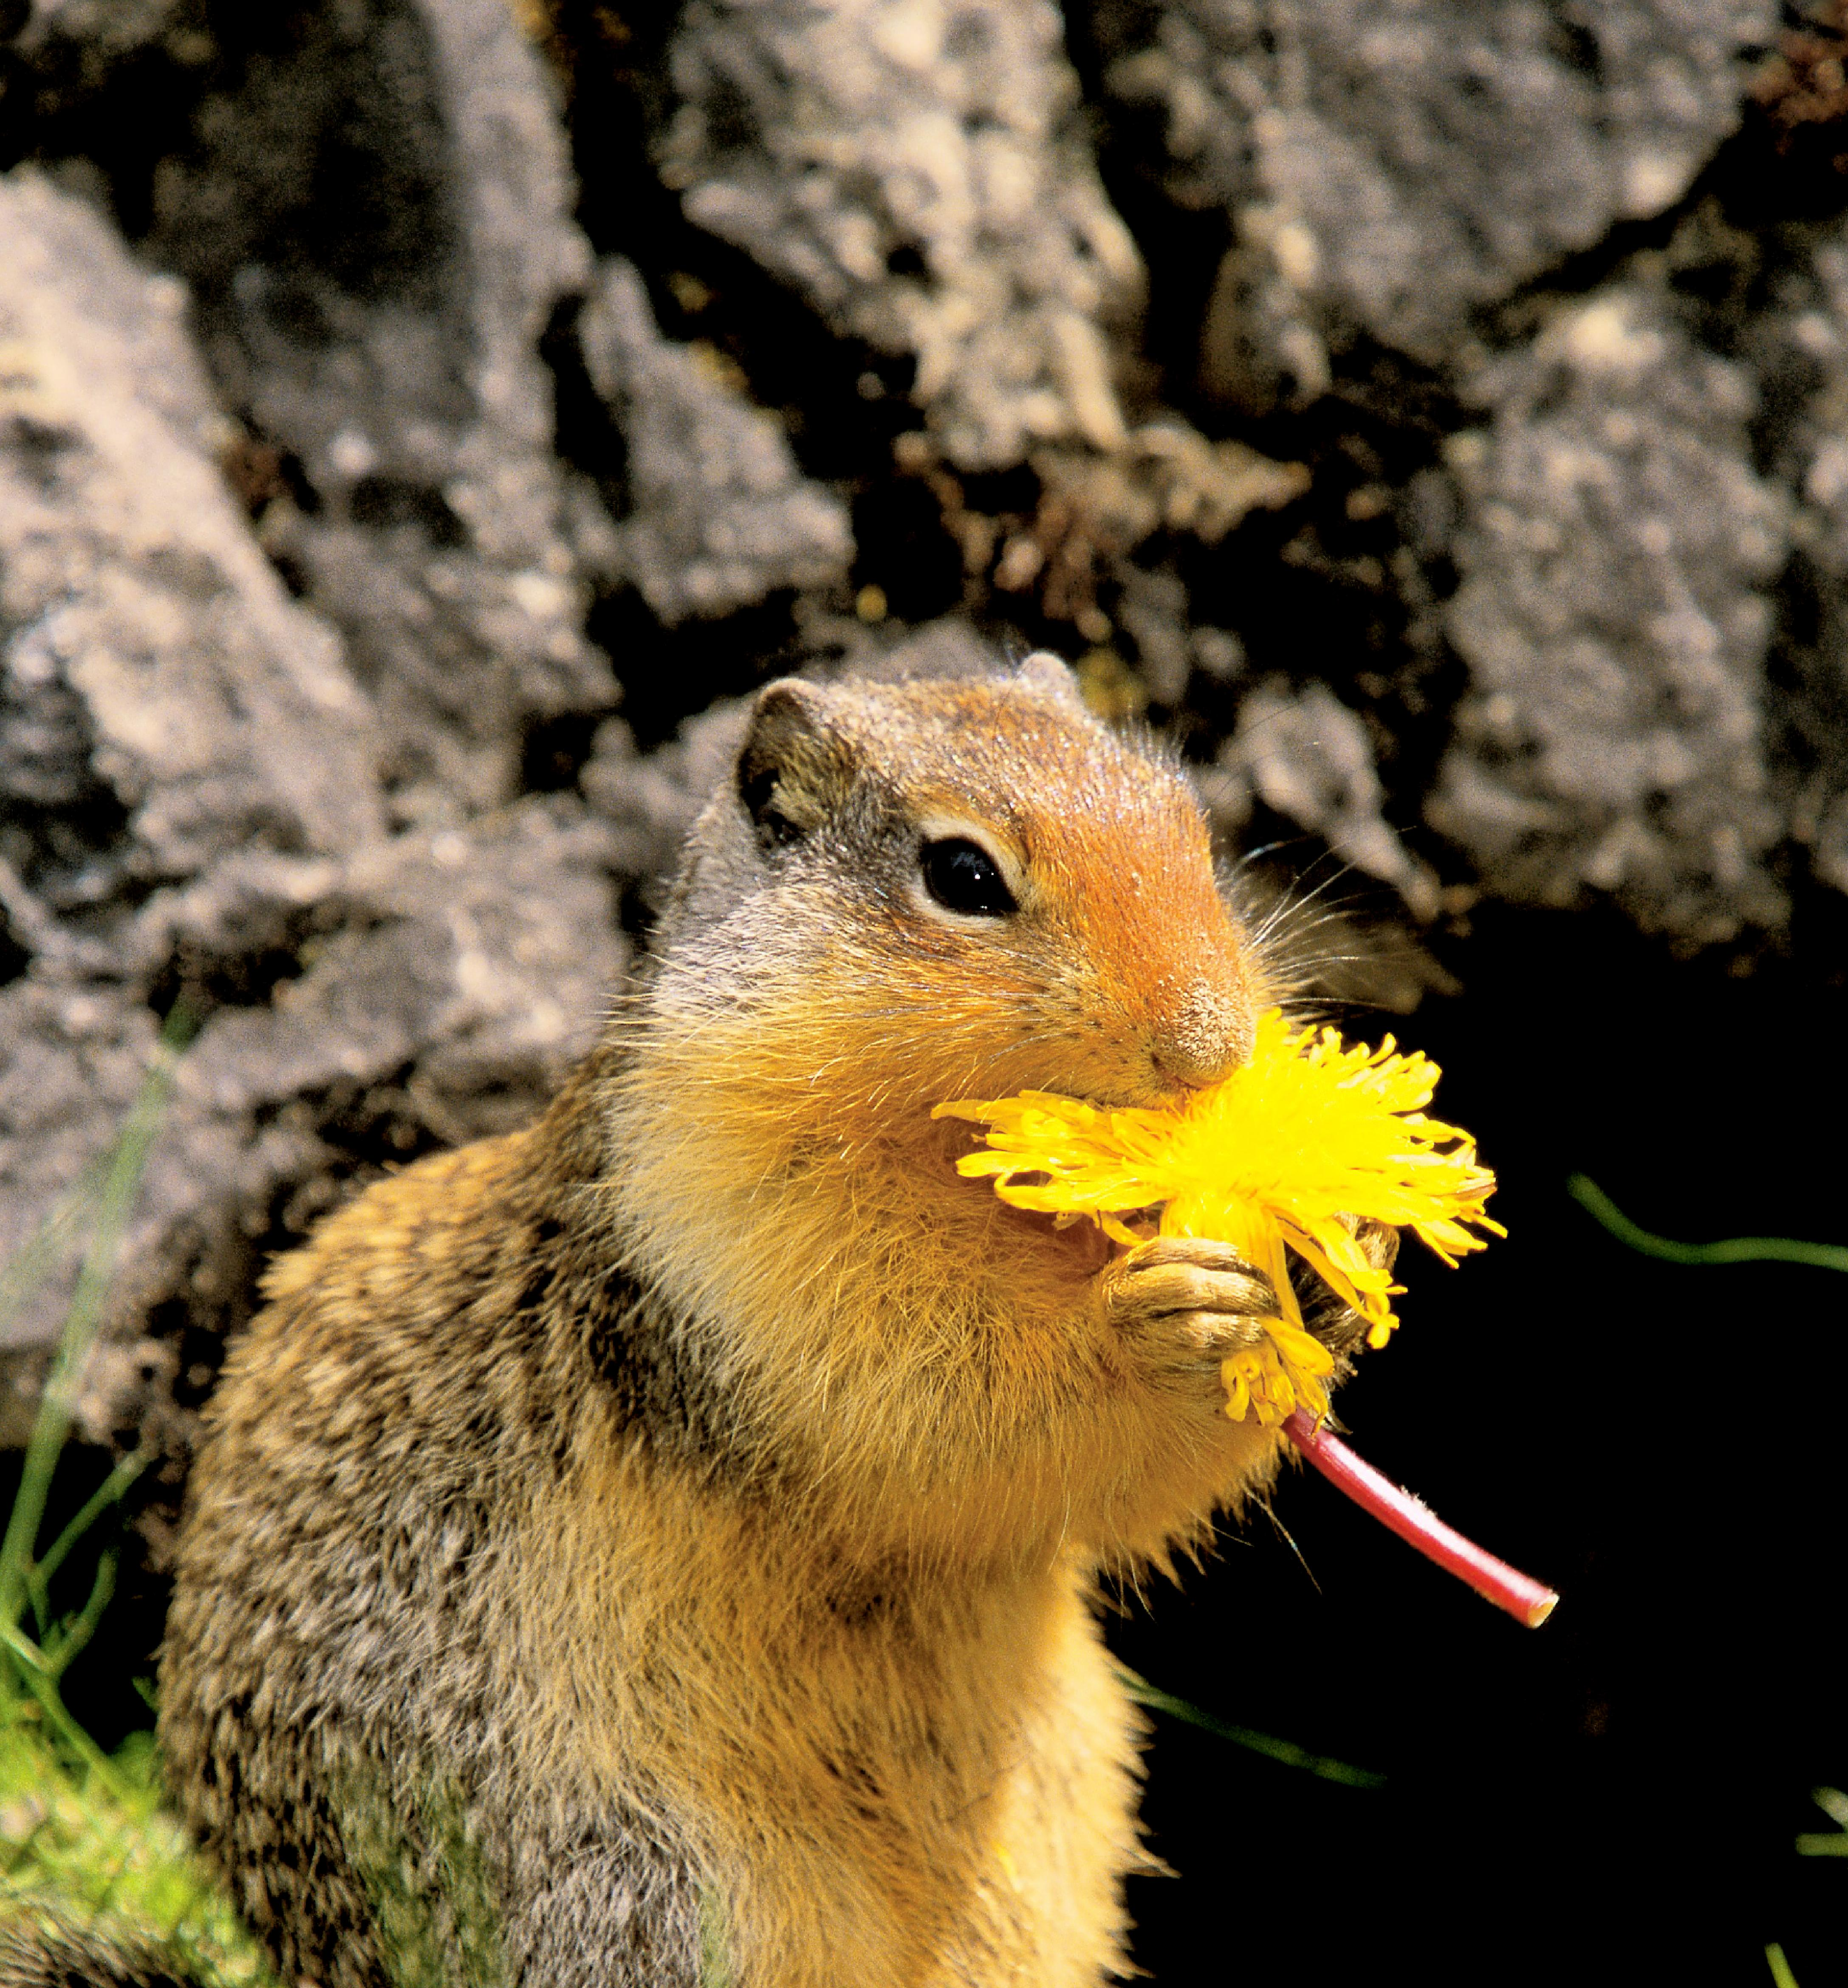
\includegraphics[width=0.60\textwidth,]{images/squirrel.jpg}%
\par

    \terminology{Linear programming} is an application of linear systems developed in the 1940s to solve complex optimization problems during wartime operations. Today, linear programming is used in scheduling and allocation of resources, in shipping and telecommunications networks, and in the selection of stocks and bonds for portfolios. In 1980, the computer scientist Laszlo Lovasz said, ``If one would take statistics about which mathematical problem is using up most of the computer time in the world, ... the answer would probably be linear programming.'' 
%
\par

	George Dantzig (1914–2005) invented the simplex method for solving linear programming problems in 1947. His first application of the method was to determine an adequate diet of least cost. This problem involved 9 equations in 77 unknowns and took 120 days to solve using the desk calculators available at the time. In this chapter, we use a graphing technique to solve problems in two unknowns. For example, the diet of the Columbian ground squirrel consists of two foods: grass and forb (a type of flowering weed). Small animals spend most of their time foraging for food, but they must also be alert for predators. Which foraging strategy favors survival: Should the squirrel try to satisfy its dietary requirements in minimum time, thus minimizing its exposure to predators and the elements, or should it try to maximize its intake of nutrients?
%
\leavevmode%
\begin{figure}
\centering
\pushValignCaptionBottom[b]{minipage}{.50\textwidth}{%
\centering% horizontal alignment 
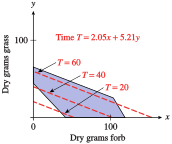
\includegraphics[width=\textwidth,]{images/fig-minimize-time-eating.pdf}}% end body 
{}% caption 
\pushValignCaptionBottom[b]{minipage}{.50\textwidth}{%
\centering% horizontal alignment 
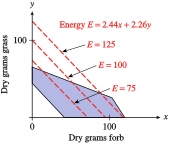
\includegraphics[width=\textwidth,]{images/fig-maximize-energy.pdf}}% end body 
{}% caption 
\popValignCaptionBottom
\end{figure}
\par

	Using linear programming, Gary Belovsky of Notre Dame University identified the optimal amounts of forb and grass for each foraging strategy. We can compare those solutions to the squirrel's actual diet to see which strategy the squirrel favors.
%
\begin{investigation}[Interpolating Polynomials]\label{investigation-1}

	In {$\langle\langle$chap6$\rangle\rangle$}, we learned to fit a quadratic function through three points on its graph. A polynomial whose graph passes through a given set of points is called an \terminology{interpolating polynomial}. Because polynomials are easy to evaluate and manipulate, they are often used to approximate more complicated functions and to describe the shapes of curves.
%
\par

	In this Investigation, we find interpolating polynomials of degrees \(1\), \(2\), and \(3\) to approximate the function \(f(x) = \frac{12}{x}\).
%
\par

	\leavevmode%
\begin{enumerate}[label=*\arabic**]
\item\hypertarget{li-1}{}\begin{enumerate}[label=*\alph**]
\item\hypertarget{li-2}{}
					Graph the function \(f(x) = \frac{12}{x}\) in the window
					\begin{align*}

							\text{Xmin} \amp = -2 \amp\amp \text{Xmax} = 7.4
						\\

							\text{Ymin} \amp = -5 \amp\amp \text{Ymax} = 20
						
\end{align*}
				%
\item\hypertarget{li-3}{}
					Complete the table of values.
					\begin{tabular}{AcAcAcAcAcAcAcA}\hrulethick
\(x\)&\(1\)&\(2\)&\(3\)&\(4\)&\(5\)&\(6\)\tabularnewline\hrulethin
\(f(x)\)&\(\hphantom{0000}\)&\(\hphantom{0000}\)&\(\hphantom{0000}\)&\(\hphantom{0000}\)&\(\hphantom{0000}\)&\(\hphantom{0000}\)\tabularnewline\hrulethin
\end{tabular}

				%
\end{enumerate}
\item\hypertarget{li-4}{}
			First we will find a linear polynomial \(P_1(x) = ax + b\) that matches \(f(x)\) at \(x = 1\) and \(x=6\). We must find constants \(a\) and \(b\) so that \(P_1(1) = f(1)\) and \(P_1(6) = f(6)\).
			\begin{enumerate}[label=*\alph**]
\item\hypertarget{li-5}{}
					The two conditions above translate into equations about \(a\) and \(b\). The constants \(a\) and \(b\) must satisfy the system
					\begin{align*}
a \cdot 1 + b \amp = f (1)\\
a \cdot 6 + b \amp = f (6)
\end{align*}
					Solve the system and find the polynomial \(P_1(x)\).
				%
\item\hypertarget{li-6}{}
					Graph \(P_1(x)\) in the same window with \(f(x)\).
				%
\end{enumerate}
\item\hypertarget{li-7}{}
			Next, we will find a quadratic polynomial \(P_2(x) = ax^2 + bx + c\) that matches \(f(x)\) at \(x = 1\), \(2.5\), and \(6\).
			\begin{enumerate}[label=*\alph**]
\item\hypertarget{li-8}{}
					Write and solve a system of equations for the constants \(a\), \(b\), and \(c\).
				%
\item\hypertarget{li-9}{}
					Graph \(P_2(x)\) in the same window with \(f(x)\).
				%
\end{enumerate}

		%
\item\hypertarget{li-10}{}
			We can also find a cubic polynomial \(P_3(x) = ax^3 + bx^2 + cx + d\) that matches \(f(x)\) at \(x = 1\), \(3\), \(4\), and \(6\).
			\begin{enumerate}[label=*\alph**]
\item\hypertarget{li-11}{}
					Write a system of equations for \(a\), \(b\), \(c\), and \(d\). We will see how to solve such a system later in this chapter. For now, we will use the calculator's cubic regression feature.
				%
\item\hypertarget{li-12}{}
					Enter the coordinates of \(P_3(x)\) evaluated at \(x=1\), \(3\), \(4\), and \(6\) into \(L_1\) and \(L_2\) under the \emph{STAT EDIT} menu. Then, from the \emph{STAT CALC} menu, choose \emph{6: CubicReg} and press \lstinline?ENTER?.
				%
\item\hypertarget{li-13}{}
					Graph \(P_3(x)\) in the same window with \(f(x)\).
				%
\end{enumerate}

		%
\item\hypertarget{li-14}{}
			How well does each interpolating polynomial approximate the function \(f(x)\)? Graph the "error function," \(E_n(x)\), for each polynomial on the interval \([−2, 7.4]\).
			\begin{align*}
E_1(x) \amp = f(x) − P_1(x)\\
E_2(x) \amp = f(x) − P_2(x)\\
E_3(x) \amp = f(x) − P_3(x)
\end{align*}
			(You will have to choose a suitable \(y\)-window for each error function.) What is the maximum error on the interval \([−2, 7.4]\) for each approximating polynomial?
		%
\end{enumerate}

%
\end{investigation}
\typeout{************************************************}
\typeout{Section 1.1 Systems of Linear Equations in Two Variables}
\typeout{************************************************}
\section[Systems of Linear Equations in Two Variables]{Systems of Linear Equations in Two Variables}\label{Systems-of-Linear-Equations-in-Two-Variables}

	Systems of linear equations are some of the most useful and widely used mathematical tools for solving problems. Systems involving hundreds of variables and equations are not uncommon in applications such as scheduling airline flights or routing telephone calls.
%
\typeout{************************************************}
\typeout{Subsection 1.1.1 Solving Systems by Graphing}
\typeout{************************************************}
\subsection[Solving Systems by Graphing]{Solving Systems by Graphing}\label{subsection-1}

	A biologist wants to know the average weights of two species of birds in a wildlife preserve. She sets up a feeder whose platform is actually a scale and mounts a camera to monitor the feeder. She waits until the feeder is occupied only by members of the two species she is studying, robins and thrushes. Then she takes a picture, which records the number of each species on the scale and the total weight registered.
%
\par

	From her two best pictures, she obtains the following information. The total weight of three thrushes and six robins is \(48\) ounces, and the total weight of five thrushes and two robins is \(32\) ounces. Using these data, the biologist estimates the average weight of a thrush and of a robin. She begins by assigning variables to the two unknown quantities:
	\begin{align*}

			\amp\text{Average weight of a thrush:} ~~t			
		\\

			\amp\text{Average weight of a robin:} ~~r			
		
\end{align*}
%
\par

	Because there are two variables, the biologist must write two equations about the weights of the birds. In each of the two photos,
	\begin{equation*}
		(\text{weight of thrushes}) + (\text{weight of robins}) = \text{total weight}
	\end{equation*}
	Thus,
	\begin{alignat*}{3}
3t \amp {}+{} \amp  6r  {}\amp={} \amp 48\\
5t \amp {}+{} \amp 2r  {}\amp={} \amp 32
\end{alignat*}
%
\leavevmode%
\begin{figure}
\centering
\pushValignCaptionBottom[c]{minipage}{.60\textwidth}{%
\parbox{\textwidth}{%
% horizontal alignment 

	This pair of equations is an example of a \terminology{linear system} \terminology{of two equations in two unknowns} (or a \(2\times 2\) linear system, for short). A \terminology{solution} to the system is an ordered pair of numbers, \((t, r)\), that satisfies both equations in the system.
}%
}% end body 
{}% caption 
\pushValignCaptionBottom[c]{minipage}{.40\textwidth}{%
\centering% horizontal alignment 
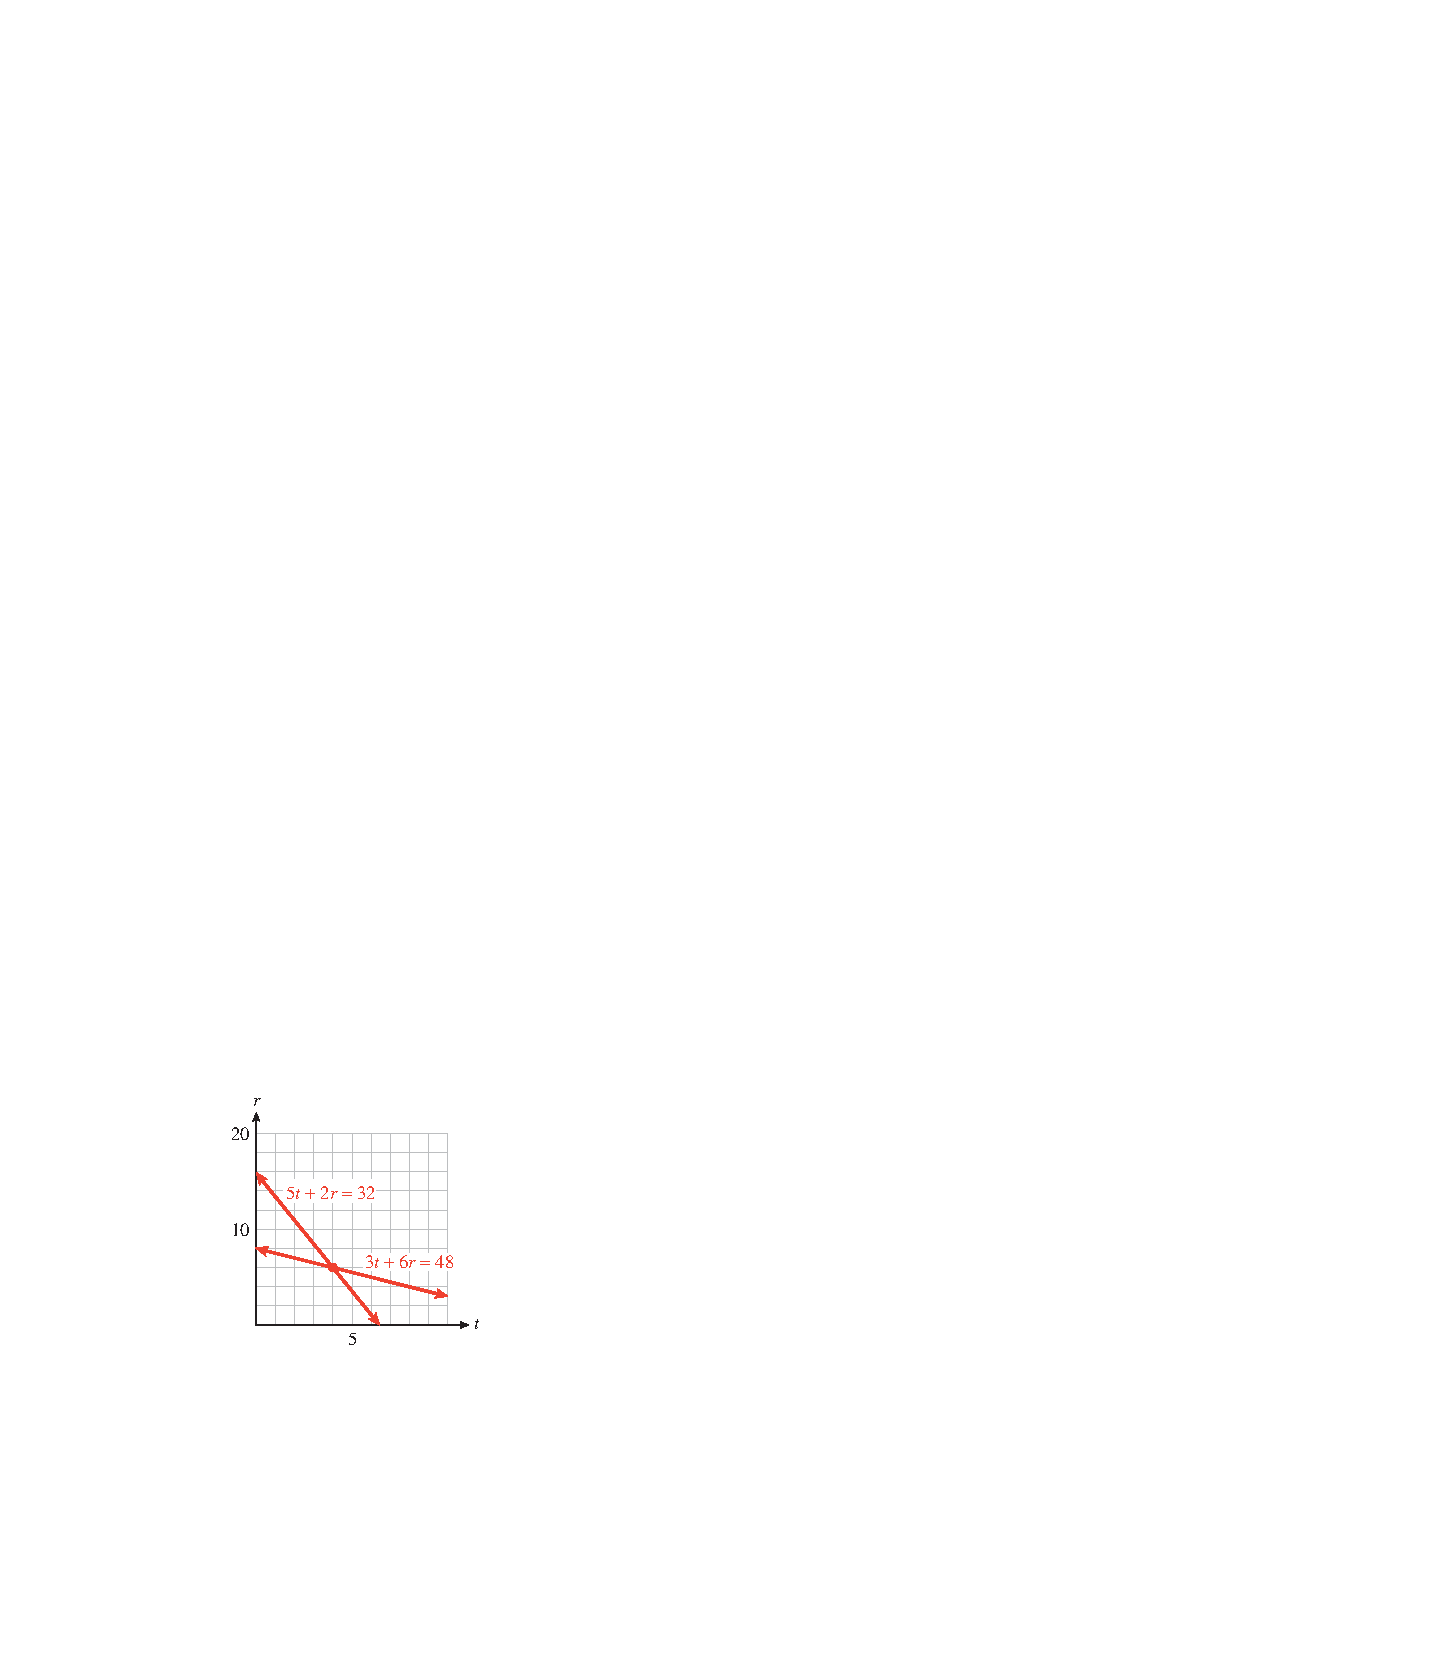
\includegraphics[width=\textwidth,]{images/fig-2x2-linear-system.pdf}}% end body 
{\captionof{figure}{\label{fig-2x2-linear-system}}
}% caption 
\popValignCaptionBottom
\end{figure}
\par

	Recall that every point on the graph of an equation represents a solution to that equation. A solution to \emph{both} equations corresponds to a point on both graphs. Therefore, a solution to the system is a point where the two graphs intersect. From \hyperref[fig-2x2-linear-system]{Figure~\ref{fig-2x2-linear-system}}, it appears that the intersection point is \((4, 6)\), so we expect that the values \(t=\alert{4}\) and \(r=\blert{6}\) form the solution to the system. We can check by verifying that these values satisfy \emph{both} equations in the system.
	\begin{align*}

			3(\alert{4}) + 6(\blert{6})\amp\stackrel{?}{=}48 \amp\amp\text{True}
		\\

			5(\alert{4}) + 2(\blert{6})\amp\stackrel{?}{=}32 \amp\amp\text{True}
		
\end{align*}
	Both equations are true, so we conclude that the average weight of a thrush is \(4\) ounces, and the average weight of a robin is \(6\) ounces.
%
\par

	We can obtain graphs for the equations in a system quickly and easily using a calculator.
%
\begin{example}[]\label{example-GC-2x2-system}

		Use your calculator to solve the system by graphing.
		\begin{align*}

				y \amp = 1.7x + 0.4
			\\

				y \amp = 4.1x + 5.2
			
\end{align*}
	%
\par\medskip\noindent%
\textbf{Solution.}\quad 
		Set the graphing window to
		\begin{align*}

				\text{Xmin} \amp = -9.4 \amp\amp \text{Xmax} = 9.4
			\\

				\text{Ymin} \amp = -10 \amp\amp \text{Ymax} = 10
			
\end{align*}
		and enter the two equations We can see in \hyperref[fig-GC-2x2-system]{Figure~\ref{fig-GC-2x2-system}} that the two lines intersect in the third quadrant. Use the \lstinline?TRACE? key or the \emph{intersect} feature to find the coordinates of the intersection point. Check that the point \((−2,−3)\) lies on both graphs. The solution to the system is \(x = −2\), \(y=-3\).
		\leavevmode%
\begin{figure}
\centering
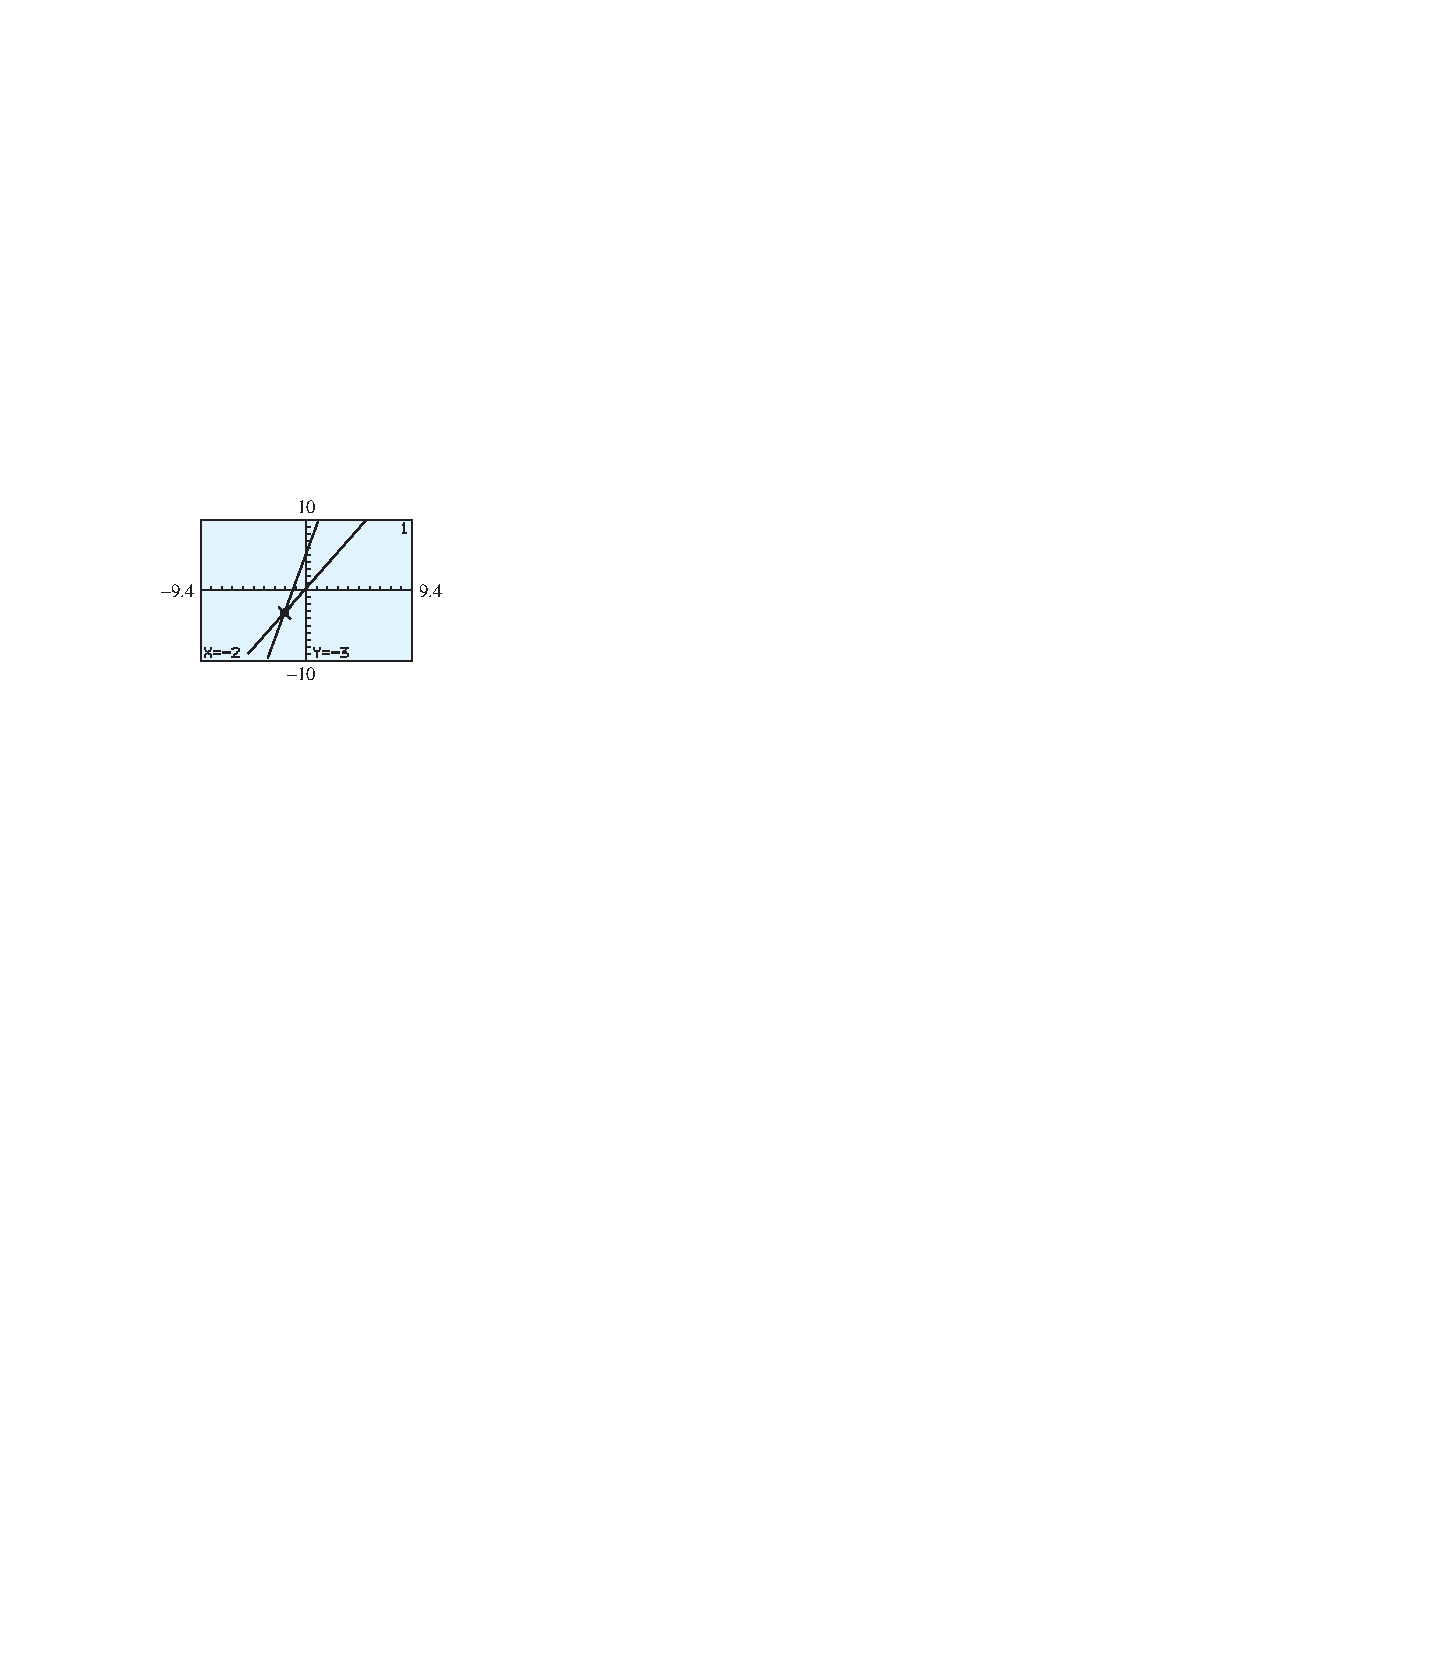
\includegraphics[width=0.60\textwidth,]{images/fig-GC-2x2-system.pdf}\caption{\label{fig-GC-2x2-system}}
\end{figure}

	%
\end{example}
\par

	The values we obtain from a calculator may be only approximations, so it is a good idea to check the solution algebraically. In \hyperref[example-GC-2x2-system]{Example~\ref{example-GC-2x2-system}}, we find that both equations are true when we substitute \(x = \alert{−2}\) and \(y=\blert{-3}\).
	\begin{align*}

			\blert{-3}\amp = 1.7(\alert{-2})+0.4\amp\amp\text{True}
		\\

			\blert{-3}\amp = 4.2(\alert{-2})+5.2\amp\amp\text{True}
		
\end{align*}
%
\begin{exercise}\label{exercise-1}

		\leavevmode%
\begin{enumerate}[label=*\alph**]
\item\hypertarget{li-15}{}
				Solve the system of equations
				\begin{align*}

						y \amp = −0.7x + 6.9
					\\

						y \amp =1.2x − 6.4
					
\end{align*}
				by graphing. Use the window
				\begin{align*}

						\text{Xmin} \amp = -9.4 \amp\amp \text{Xmax} = 9.4
					\\

						\text{Ymin} \amp = -10 \amp\amp \text{Ymax} = 10
					
\end{align*}
			%
\end{enumerate}

	%
\end{exercise}
\begin{remark}[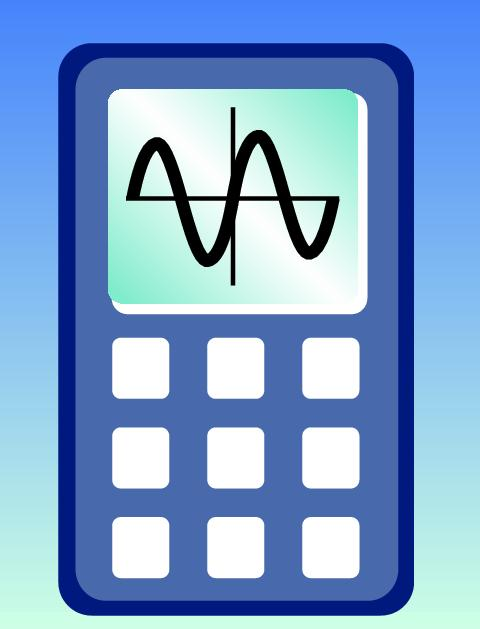
\includegraphics[width=0.8\textwidth,]{images/icon-GC.jpg}Using the Intersect Feature to Solve a System]\label{remark-1}

	Because the \lstinline?TRACE? feature does not show every point on a graph, we may not find the exact solution to a system by tracing the graphs.
%
\end{remark}
\begin{example}[]\label{example-2}

		Solve the system
		\begin{align*}

				3x − 2.8y \amp= 21.06
			\\

				2x + 1.2y \amp= 5.3
			
\end{align*}
	%
\par\medskip\noindent%
\textbf{Solution.}\quad 
		We can graph this system in the standard window by solving each equation for \(y\). Enter
		\begin{align*}

				Y_1\amp = (21.06 − 3X)/−2.8
			\\

				Y_2\amp  = (5.3 − 2X)/1.2
			
\end{align*}
		and then press \lstinline?ZOOM? \(6\). (Do not forget the parentheses around the numerator of each expression.) Trace along the first line to find the intersection point. It appears to be at \(x=4.468051\), \(y =-2.734195\), as shown in \hyperref[fig-GC-2x2-system2]{Figure~\ref{fig-GC-2x2-system2}}a. However, if we press the up or down arrow to read the coordinates off the second line, we see that for the same \(x\)-coordinate we obtain a different \(y\)-coordinate, as in \hyperref[fig-GC-2x2-system2]{Figure~\ref{fig-GC-2x2-system2}}b. The different \(y\)-coordinates indicate that we have not found an intersection point, although we are close. However, the intersect feature can give us a better estimate, \(x = 4.36\), \(y = −2.85\).
		\leavevmode%
\begin{figure}
\centering
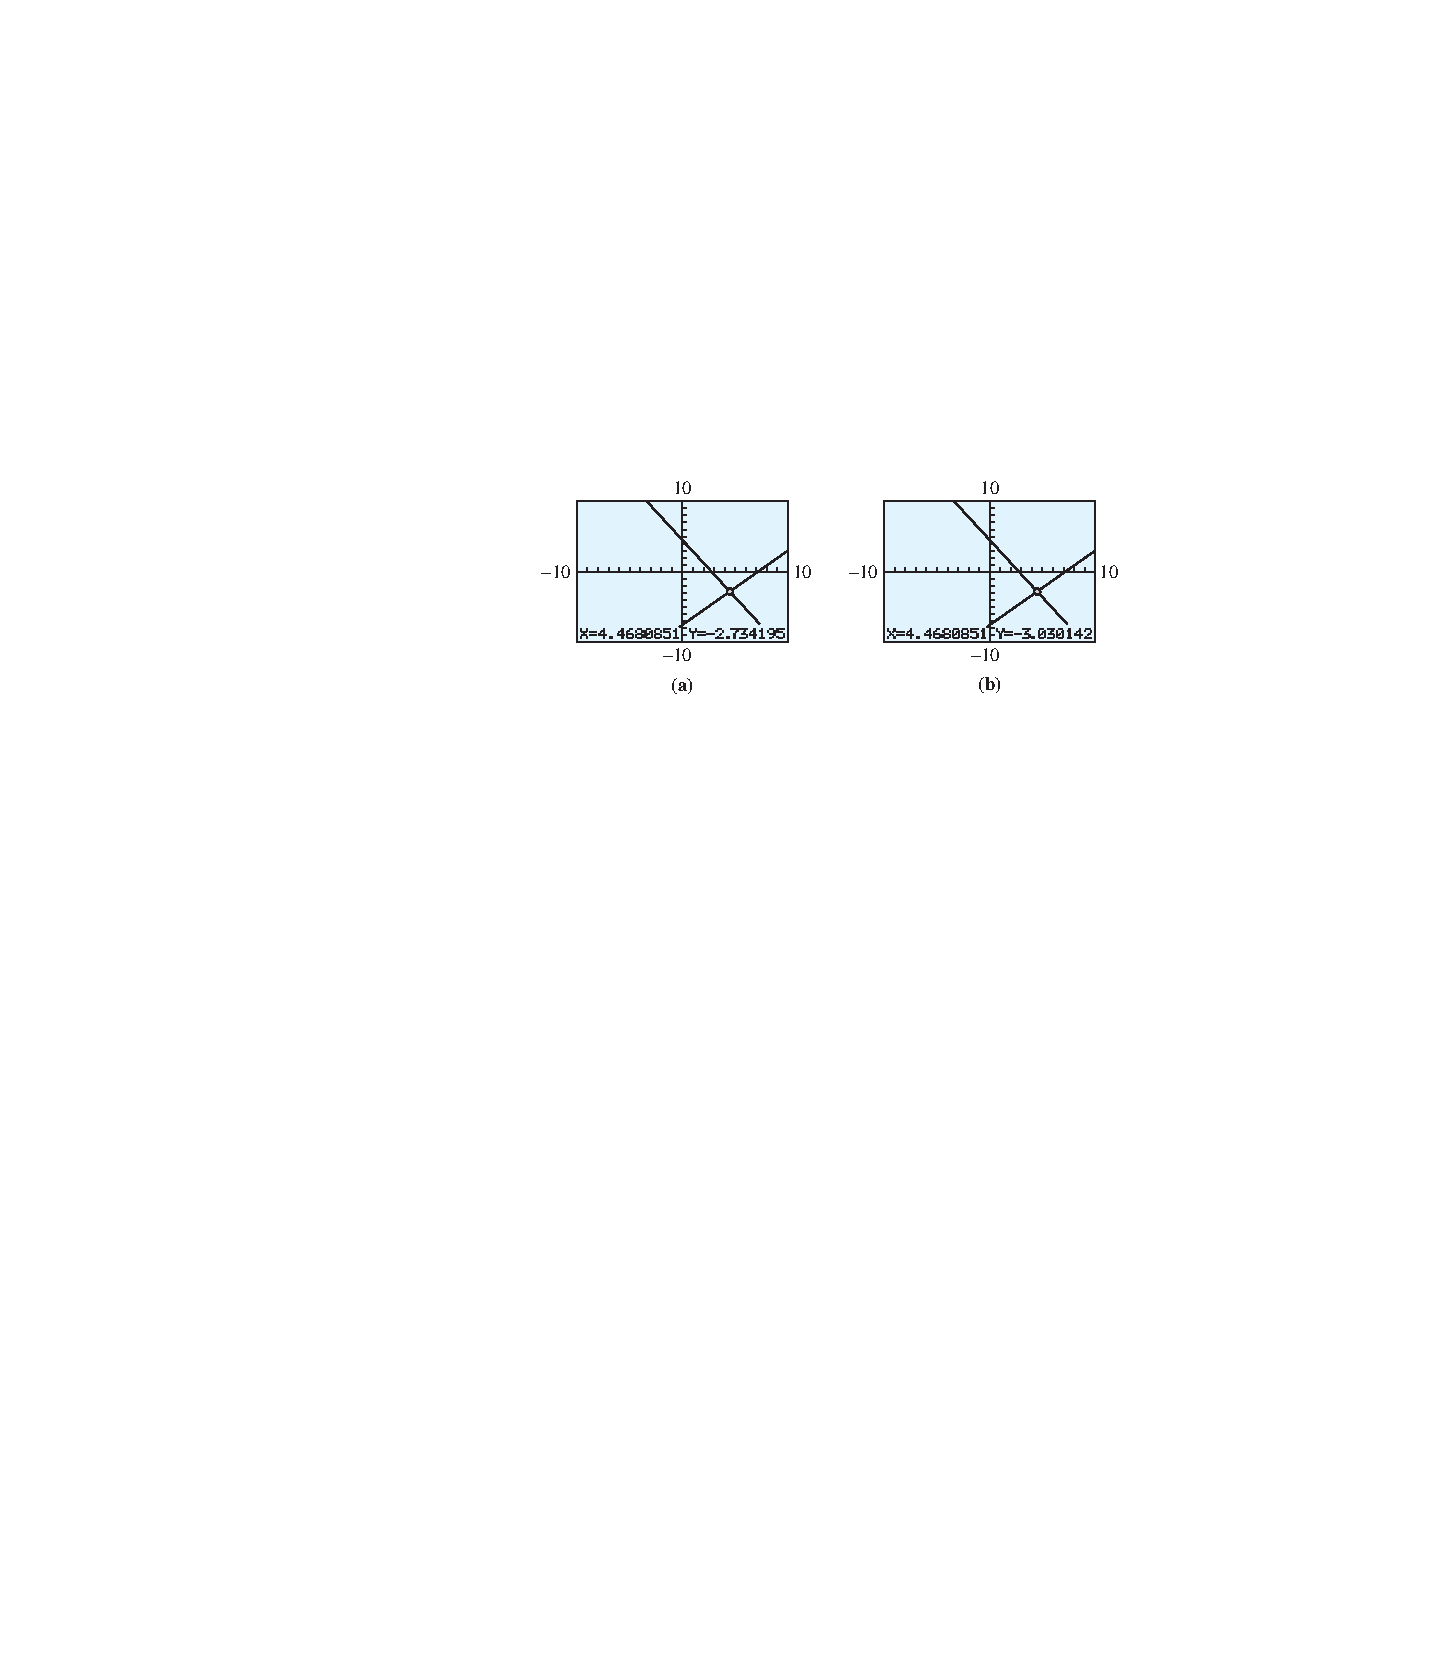
\includegraphics[width=0.100\textwidth,]{images/fig-GC-2x2-system2.pdf}\caption{\label{fig-GC-2x2-system2}}
\end{figure}

		We can substitute these values into the original system to check that they satisfy both equations.
		\begin{align*}

				3(\alert{4.36}) − 2.8(\blert{−2.85}) \amp = 21.06
			\\

				2(\alert{4.36}) + 1.2(\blert{−2.85}) \amp = 5.3
			
\end{align*}
	%
\end{example}
\begin{exercise}\label{exercise-2}

		Solve the system of equations
		\begin{gather*}

				y = 47x − 1930
			\\

				y + 19x = 710
			
\end{gather*}
		by graphing. Use the \emph{intersect} feature in the window
		\begin{align*}

				\text{Xmin} \amp = 0 \amp\amp \text{Xmax} = 94
			\\

				\text{Ymin} \amp = -2000 \amp\amp \text{Ymax} = 1000
			
\end{align*}
	%
\end{exercise}
\par

	In previous algebra courses, you learned two algebraic techniques for solving \(2\times 2\) linear systems: \terminology{substitution} and \terminology{elimination}. See Algebra Skills Refresher \hyperref[appendix-Linear-Systems-in-Two-Variables]{\ref{appendix-Linear-Systems-in-Two-Variables}} if you would like to review these techniques.
%
\begin{example}[]\label{example-3}

		Rani kayaks downstream for \(45\) minutes and travels a distance of \(6000\) meters. On the return journey upstream, she covers only \(4800\) meters in \(45\) minutes. How fast is the current in the river, and how fast would Rani kayak in still water? (Give your answers in meters per minute.)
	%
\par\medskip\noindent%
\textbf{Solution.}\quad 
		\leavevmode%
\begin{description}
\item[Step 1: ]{}
				\begin{tabular}{ll}
Rani's speed in still water:%
&\(r\)\tabularnewline[0pt]
Speed of the current:%
&\(s\)
\end{tabular}

			%
\item[Step 2:]{}
				We must write two equations using the variables \(r\) and \(s\). First, organize the information into a table. When Rani travels downstream, the current in the river helps her, so her effective speed is \(r+s\). When she travels upstream she is fighting the current, so her speed is actually \(r-s\).
				\begin{tabular}{AlAcAcAcA}\hrulethin
%
&Rate%
&Time%
&Distance%
\tabularnewline\hrulethin
Downstream%
&\(r+s\)&\(45\)&\(6000\)\tabularnewline\hrulethin
Upstream%
&\(r-s\)&\(45\)&\(4800\)\tabularnewline\hrulethin
\end{tabular}

				Using the formula \(\text{rate} \times \text{time} = \text{distance}\), we write one equation describing Rani's journey downstream, and a second equation for the journey upstream.
				\begin{align*}

						(r + s) \cdot 45 \amp = 6000
					\\

						(r − s) \cdot 45 \amp = 4800
					
\end{align*}
				Apply the distributive law to write each equation in standard form.
				\begin{align*}

						45r + 45s \amp = 6000 \amp\amp(1)
					\\

						45r − 45s \amp = 4800 \amp\amp(2)
					
\end{align*}
			%
\item[Step 3:]{}
				To solve the system, we eliminate the variable \(s\) by adding the two equations vertically.
				\leavevmode%
\begin{table}
\centering
\begin{tabular}{rrrrr}
\(45r\)&\(+\)&\(45s\)&\(=\)&\(-6000\)\tabularnewline[0pt]
\(+45r\)&\(-\)&\(45s\)&\(=\)&\(4800\)\tabularnewline\hrulethin
\(90r\)&\(\)&\(\)&\(=\)&\(10,800\)
\end{tabular}
\end{table}

				We now have an equation in one variable only, which we can solve for \(r\).
				\begin{align*}

						90r \amp = 10,800\amp\amp\text{Divide both sides by 90.}
					\\

						r \amp = 120
					
\end{align*}
				To solve for \(s\) we substitute \(r = 120\) into any previous equation involving both \(r\) and \(s\). We will use Equation (1).
				\begin{align*}

						45(120) + 45s\amp = 6000 \amp\amp\text{Simplify the left side.}
					\\

						5400 + 45s \amp = 6000 \amp\amp\text{Subtract 5400 from both sides.}
					\\

						45s \amp = 600 \amp\amp\text{Divide both sides by 45; reduce.}
					\\

						s\amp = \frac{40}{3}
					
\end{align*}
			%
\item[Step 4: ]{}
				The speed of the current is \(\frac{40}{3}\), or \(13\frac{1}{3} \) meters per minute, and Rani's speed in still water is \(120\) meters per minute.
			%
\end{description}

	%
\end{example}
\begin{exercise}\label{exercise-3}

		It took Leon \(7\) hours to fly the same distance that Marlene drove in \(21\) hours. Leon flies \(120\) miles per hour faster than Marlene drives. At what speed did each travel?
		\leavevmode%
\begin{enumerate}
\item\hypertarget{li-20}{}
				Choose variables for the unknown quantities, and fill in the table.
				\begin{tabular}{AlAcAcAcA}\hrulethin
%
&Rate%
&Time%
&Distance%
\tabularnewline\hrulethin
Leon%
&\(\)&\(\)&\(\)\tabularnewline\hrulethin
Marlene%
&\(\)&\(\)&\(\)\tabularnewline\hrulethin
\end{tabular}
\item\hypertarget{li-21}{}
				Write one equation about the Leon's and Marlene's speeds.
			%
\item\hypertarget{li-22}{}
				Write a second equation about distances.
			%
\item\hypertarget{li-23}{}
				Solve the system and answer the question in the problem.
			%
\end{enumerate}

	%
\end{exercise}
\typeout{************************************************}
\typeout{Subsection 1.1.2 Inconsistent and Dependent Systems}
\typeout{************************************************}
\subsection[Inconsistent and Dependent Systems]{Inconsistent and Dependent Systems}\label{subsection-2}

	Because two straight lines do not always intersect at a single point, a \(2\times 2\) system of linear equations does not always have a unique solution. In fact, there are three possibilities, as illustrated in \hyperref[fig-3-cases-2x2-systems]{Figure~\ref{fig-3-cases-2x2-systems}}.
	\leavevmode%
\begin{figure}
\centering
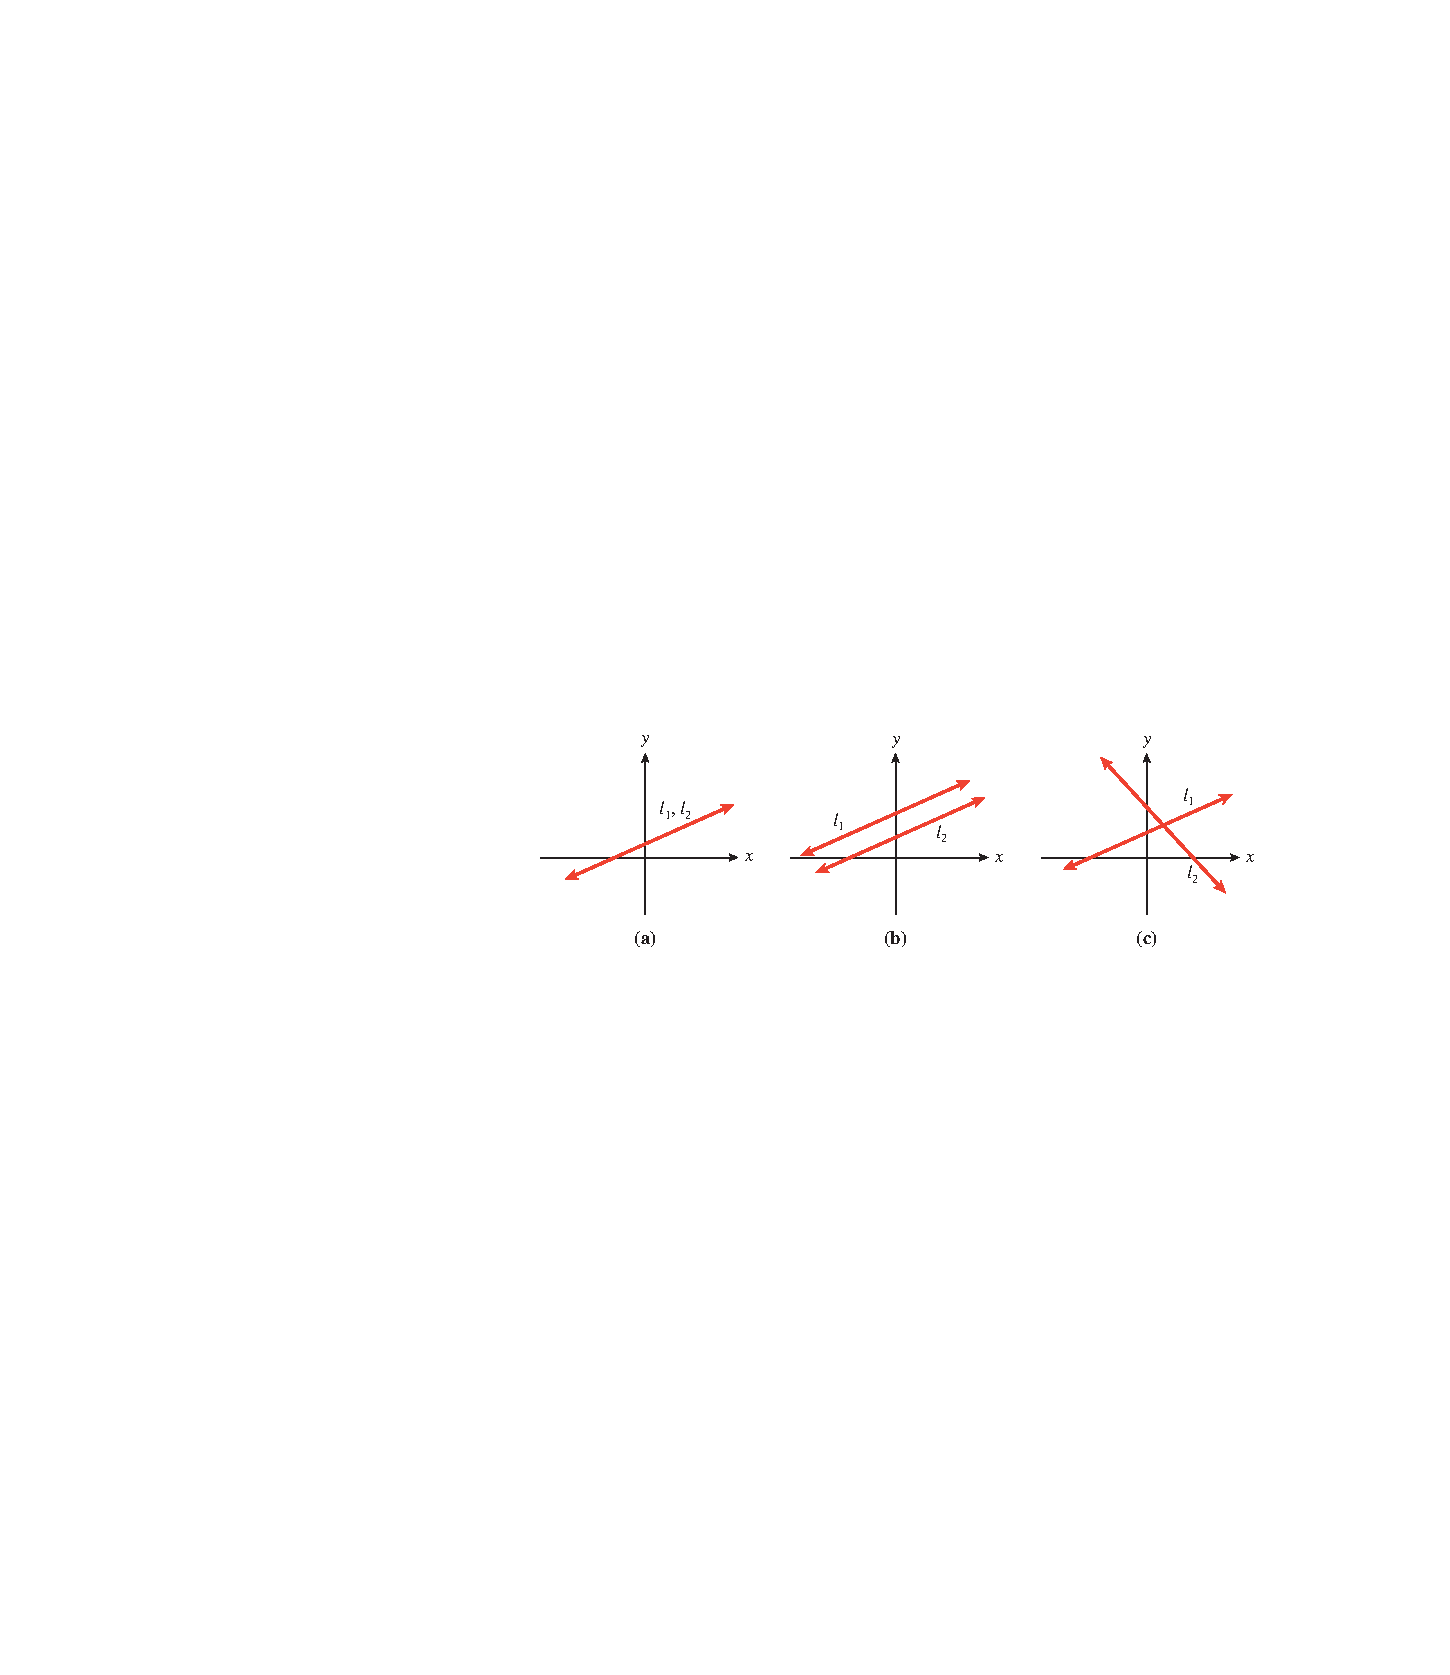
\includegraphics[,]{images/fig-3-cases-2x2-systems.pdf}\caption{\label{fig-3-cases-2x2-systems}}
\end{figure}

	\leavevmode%
\begin{enumerate}[label=*\arabic**]
\item\hypertarget{li-24}{}
			The graphs may be the same line, as shown in \hyperref[fig-3-cases-2x2-systems]{Figure~\ref{fig-3-cases-2x2-systems}}a.
		%
\item\hypertarget{li-25}{}
			The graphs may be parallel but distinct lines, as shown in \hyperref[fig-3-cases-2x2-systems]{Figure~\ref{fig-3-cases-2x2-systems}}b.
		%
\item\hypertarget{li-26}{}
			The graphs may intersect in one and only one point, as shown in \hyperref[fig-3-cases-2x2-systems]{Figure~\ref{fig-3-cases-2x2-systems}}c.
		%
\end{enumerate}

%
\begin{example}[]\label{example-inconsistent-system}

		Solve the system
		\begin{gather*}

				y = −x + 5
			\\

				2x + 2y = 3
			
\end{gather*}
	%
\par\medskip\noindent%
\textbf{Solution.}\quad 
		We use the calculator to graph both equations on the same axes, as shown in \hyperref[fig-GC-parallel-lines]{Figure~\ref{fig-GC-parallel-lines}}. First, rewrite the second equation in slope-intercept form by solving for \(y\).
		\begin{align*}

				2x + 2y \amp = 3\amp\amp\text{Substract } 2x \text{ from both sides.}
			\\

				2y \amp = −2x + 3\amp\amp\text{Divide both sides by 2.}
			\\

				y \amp = −x + 1.5
			
\end{align*}
		Now enter the equations as
		\begin{align*}

				Y_1 \amp= −X + 5
			\\

				Y_2 \amp = −X + 1.5
			
\end{align*}
		\leavevmode%
\begin{figure}
\centering
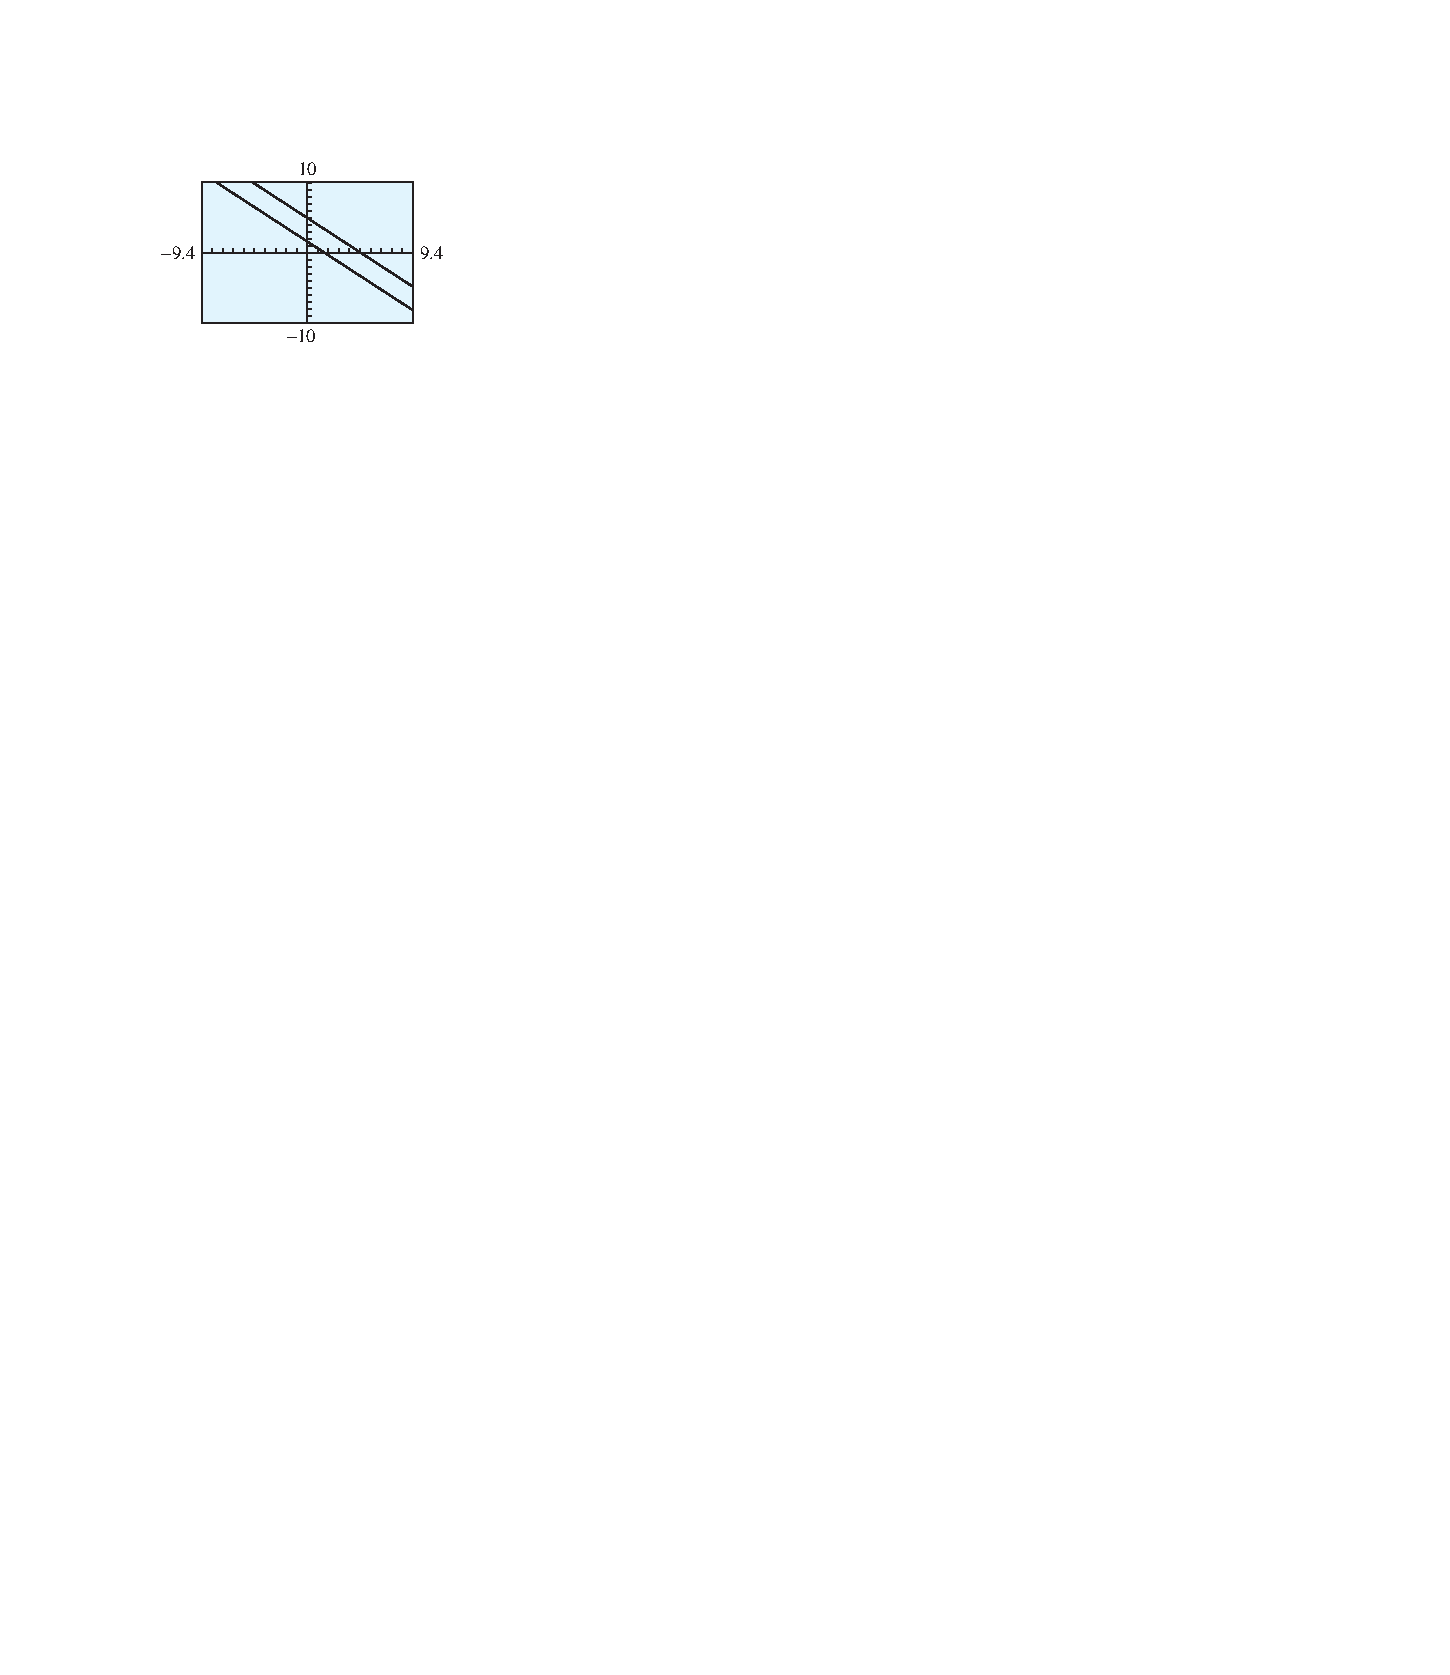
\includegraphics[width=0.50\textwidth,]{images/fig-GC-parallel-lines.pdf}\caption{\label{fig-GC-parallel-lines}}
\end{figure}

		The lines do not intersect within the viewing window; they appear to be parallel. If we look again at the equations of the lines, we recognize that both have slope \(-1\) but different \(y\)-intercepts, so they are parallel. Since parallel lines never meet, there is no solution to the system.
	%
\end{example}
\par

	A system with no solutions, such as the system in \hyperref[example-inconsistent-system]{Example~\ref{example-inconsistent-system}}, is called \terminology{inconsistent}. A \(2\times 2\) system of linear equations is inconsistent when the two equations correspond to parallel lines. This situation occurs when the lines have the same slope but different \(y\)-intercepts.
%
\begin{exercise}\label{exercise-4}

		Without graphing, show that the following system is inconsistent:
		\begin{gather*}

				3y = \frac{3}{2}x − 1
			\\

				2x − 4y = 3
			
\end{gather*}
	%
\end{exercise}
\par

	A linear system with infinitely many solutions is called \terminology{dependent}. A \(2\times 2\) system is dependent when the two equations actually describe the same line. This situation occurs when the two lines have the same slope \emph{and} the same \(y\)-intercept.
%
\begin{example}[]\label{example-5}

		Solve the system
		\begin{gather*}

				x = \frac{2}{3}y + 3
			\\

				3x − 2y = 9
			
\end{gather*}
	%
\par\medskip\noindent%
\textbf{Solution.}\quad 
		We begin by putting each equation in slope-intercept form.
		\begin{align*}

				x \amp = \frac{2}{3}y + 3\amp\amp\text{Subtract 3.}				
			\\

				x -3\amp = \frac{2}{3}y \amp\amp\text{Multiply by }	\frac{3}{2}.							
			\\

				\frac{3}{2}x-\frac{9}{2}\amp = y
			
\end{align*}
		For the second equation,
		\begin{align*}

				3x − 2y \amp = 9  \amp\amp\text{Subtract }	3x.
			\\

				−2y \amp = −3x + 9  \amp\amp\text{Divide by } -2.
			\\

				y \amp = \frac{3}{2}x − \frac{9}{2}
			
\end{align*}
		The two equations are actually different forms of the same equation. Because they are equivalent, they share the same line as a graph, as shown in \hyperref[fig-coincident-lines]{Figure~\ref{fig-coincident-lines}}. Every point on the first line is also a point on the second line, so every solution to the first equation is also a solution of the second equation. Thus, the system has infinitely many solutions.
		\leavevmode%
\begin{figure}
\centering
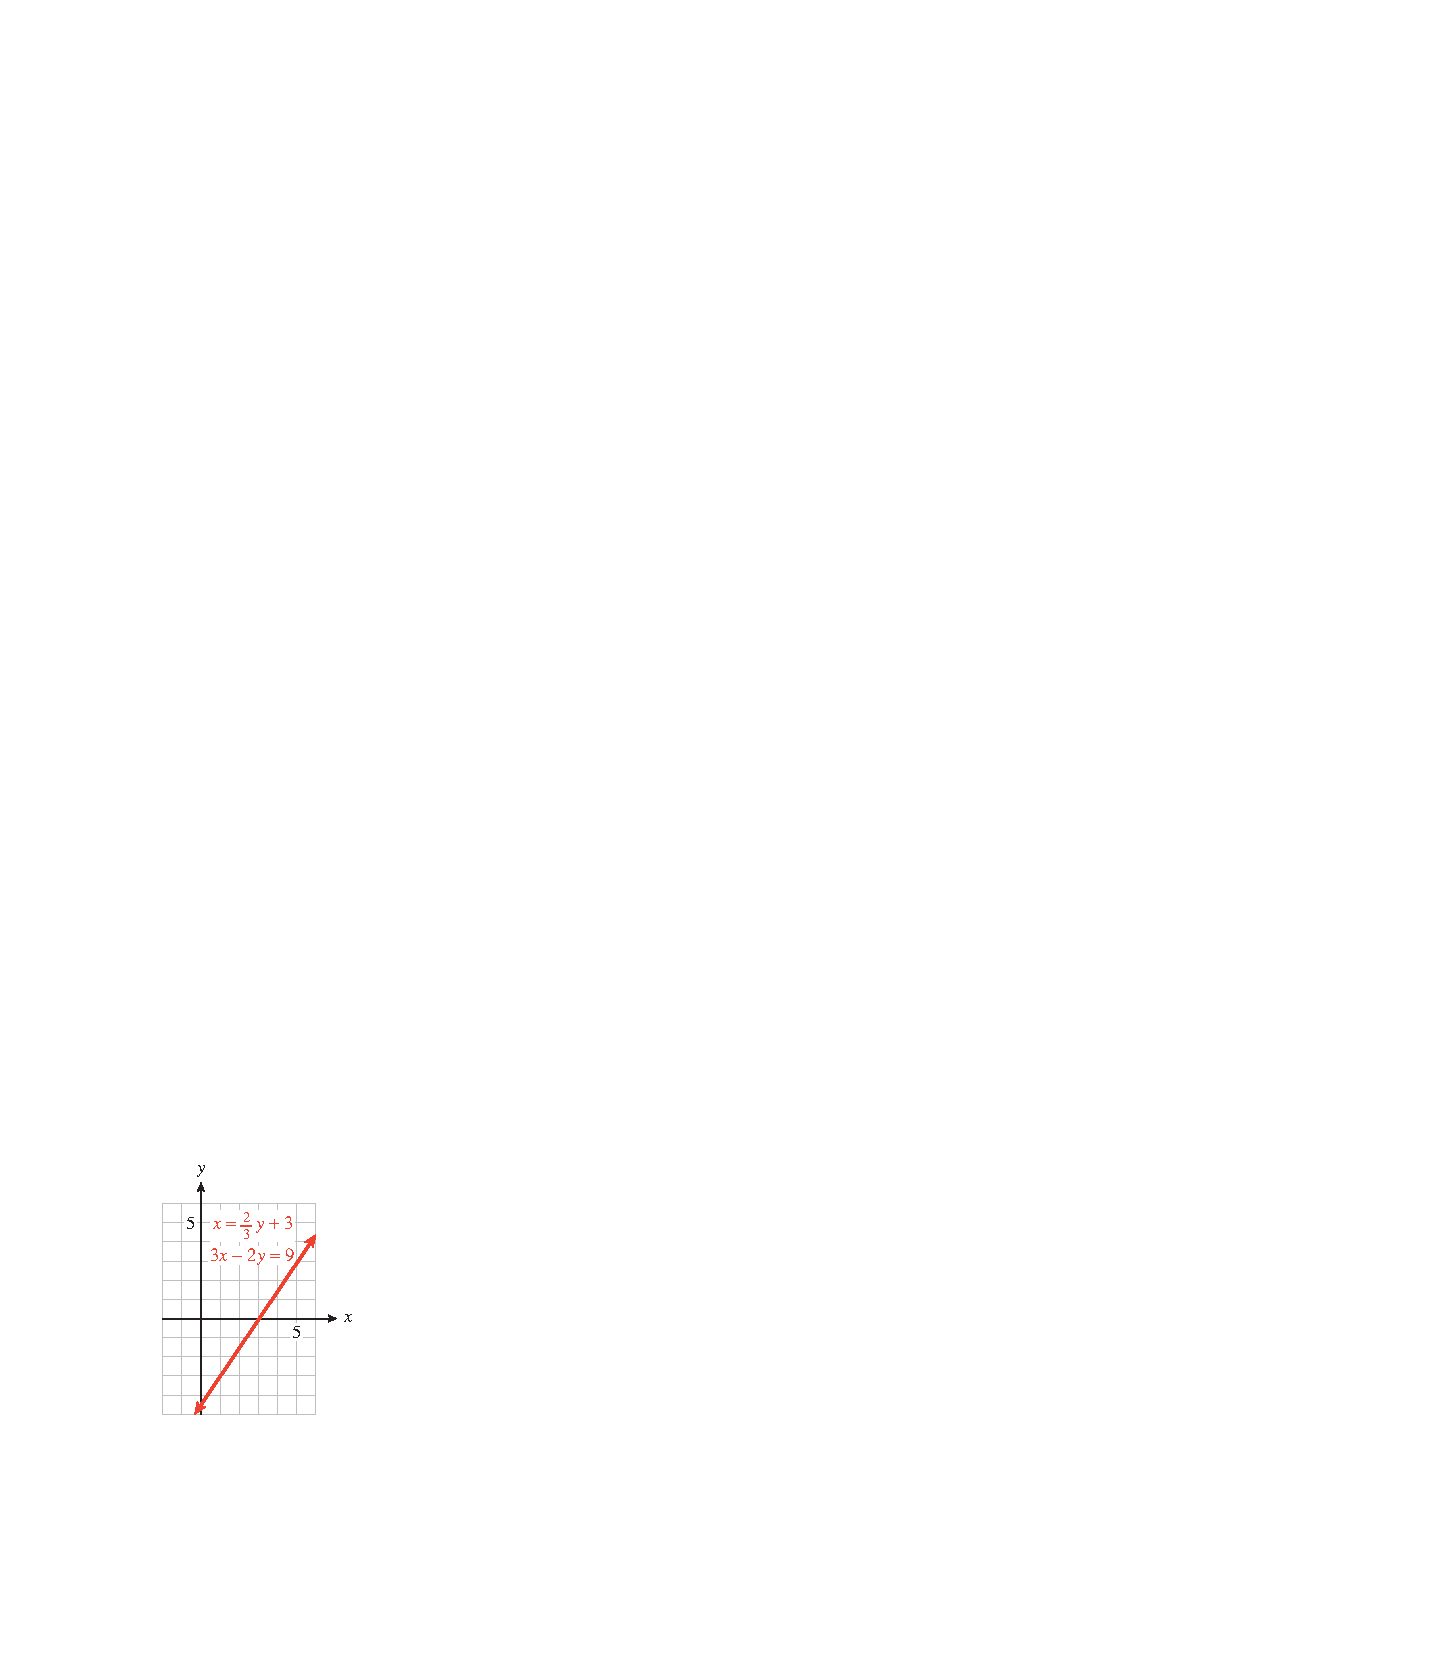
\includegraphics[width=0.40\textwidth,]{images/fig-coincident-lines.pdf}\caption{\label{fig-coincident-lines}}
\end{figure}

	%
\end{example}
\par

	Here is a summary of the three cases for a \(2\times 2\) system of linear equations.
%
\begin{assemblage}{Solutions of \(2\times 2\) Linear Systems}\label{assemblage-1}\par\medskip

	\leavevmode%
\begin{enumerate}[label=*\arabic**]
\item\hypertarget{li-27}{}
			\terminology{Dependent system}\index{}. All the solutions of one equation are also solutions to the second equation and hence are solutions of the system. The graphs of the two equations are the same line. A dependent system has infinitely many solutions.
		%
\item\hypertarget{li-28}{}
			\terminology{Inconsistent system}\index{}. The graphs of the equations are parallel lines and hence do not intersect. An inconsistent system has no solutions.
		%
\item\hypertarget{li-29}{}
			\terminology{Consistent and independent system}\index{}. The graphs of the two lines intersect in exactly one point. The system has exactly one solution.
		%
\end{enumerate}

%
\end{assemblage}
\begin{exercise}\label{exercise-5}

	\leavevmode%
\begin{enumerate}[label=*\alph**]
\item\hypertarget{li-30}{}
			Graph the system
			\begin{gather*}

					y = −3x + 6
				\\

					6x + 2y = 15
				
\end{gather*}
			by hand, using either the intercept method or the slope-intercept method. (See Sections 1.1 and 1.4 to review these methods.)
		%
\item\hypertarget{li-31}{}
			Identify the system as dependent, inconsistent, or consistent and independent.
		%
\end{enumerate}
%
\end{exercise}
\par

	It is not always easy to tell from the equations themselves whether there is one solution, no solution, or infinitely many solutions. However, the method of elimination will reveal which of the three cases applies.
%
\begin{example}[]\label{example-inconsistent-system2}

		Solve the system
		\begin{align*}

				2x \amp= 2 − 3y
			\\

				6y \amp= 7 − 4x
			
\end{align*}
	%
\par\medskip\noindent%
\textbf{Solution.}\quad 
		First, rewrite the system in standard form as
		\begin{align*}

				2x + 3y \amp = 2 \amp\amp (1)
			\\

				4x + 6y \amp = 7 \amp\amp (2)
			
\end{align*}
		Multiply Equation (1) by \(-2\) and add the result to Equation (2) to obtain
		\leavevmode%
\begin{table}
\centering
\begin{tabular}{rrrrr}
\(-4x\)&\(-\)&\(6y\)&\(=\)&\(-4\)\tabularnewline[0pt]
\(4x\)&\(+\)&\(6y\)&\(=\)&\(7\)\tabularnewline\hrulethin
\(0x\)&\(+\)&\(0y\)&\(=\)&\(3\)
\end{tabular}
\end{table}

		This equation has no solutions. The system is inconsistent. (Notice that both lines have slope \(\frac{-2}{3}\), but they have different \(y\)-intercepts, so their graphs are parallel.)
	%
\end{example}
\par

	We generalize the results from \hyperref[example-inconsistent-system2]{Example~\ref{example-inconsistent-system2}} as follows.
%
\begin{assemblage}{Inconsistent and Dependent Systems}\label{assemblage-2}\par\medskip

	\leavevmode%
\begin{enumerate}[label=*\arabic**]
\item\hypertarget{li-32}{}
			If an equation of the form
			\begin{equation*}
				0x + 0y = k \hphantom{blank}(k\ne 0)
			\end{equation*}
			is obtained as a linear combination of the equations in a system, the system is \terminology{inconsistent}.
		%
\item\hypertarget{li-33}{}
			If an equation of the form
			\begin{equation*}
				0x + 0y = 0
			\end{equation*}
			is obtained as a linear combination of the equations in a system, the system is \terminology{dependent}.
		%
\end{enumerate}

%
\end{assemblage}
\par

	\hyperref[exercise-dependent-system]{Exercise~\ref{exercise-dependent-system}} illustrates a dependent system.
%
\begin{exercise}\label{exercise-dependent-system}

		\leavevmode%
\begin{enumerate}[label=*\alph**]
\item\hypertarget{li-34}{}
				Use the method of elimination to solve the system
				\begin{align*}

						3x − 4 \amp = y
					\\

						2y + 8 \amp = 6x
					
\end{align*}
			%
\item\hypertarget{li-35}{}
				Verify that both equations have the same graph.
			%
\end{enumerate}

	%
\end{exercise}
\typeout{************************************************}
\typeout{Subsection 1.1.3 Applications}
\typeout{************************************************}
\subsection[Applications]{Applications}\label{subsection-3}

	Many practical problems involve two or more unknown quantities.
%
\begin{example}[]\label{example-7}

		A cup of rolled oats provides 11 grams of protein. A cup of rolled wheat flakes provides 8.5 grams of protein. Francine wants to combine oats and wheat to make a cereal with 10 grams of protein per cup. How much of each grain will she need in one cup of her mixture?
	%
\par\medskip\noindent%
\textbf{Solution.}\quad 
		\leavevmode%
\begin{description}
\item[Step 1:]{}
				\begin{tabular}{ll}

							Fraction of a cup of oats needed:
						%
&\(x\)\tabularnewline[0pt]

							Fraction of a cup of wheat needed:
						%
&\(y\)
\end{tabular}

			%
\item[Step 2:]{}
				Because we have two variables, we must find two equations that describe the problem. It may be helpful to organize the information into a table.
				\begin{tabular}{AlAcAcAcAcA}\hrulethin
&Cups%
&\tablecelllines{c}{m}
{Grams of protein\\
per cup}
&Grams of protein%
\tabularnewline\hrulethin
Oats%
&\(x\)&\(11\)&\(11x\)\tabularnewline\hrulethin
Wheat%
&\(y\)&\(8.5\)&\(8.5y\)\tabularnewline\hrulethin
Mixture%
&\(1\)&--&\(10\)\tabularnewline\hrulethin
\end{tabular}

				The wheat and oats together will make one cup of mixture, so the first equation is 
				\begin{equation*}
					x + y = 1
				\end{equation*}
				The \(10\) grams of protein must come form the protein in the oats plus the protein in the wheat. This gives us a second equation:
				\begin{equation*}
					11x + 8.5y = 10
				\end{equation*}
				We now have a system of equations.
			%
\item[Step 3: ]{}
				We will solve the system by graphing. First, solve each equation for \(y\) in terms of \(x\) to get
				\begin{align*}

						y \amp= −x + 1
					\\

						y \amp = (10 − 11x)/8.5
					
\end{align*}
				Although we could simplify the second equation, the calculator can graph both equations as they are. We know that x and y represent fractions of one cup, so we set the window (as shown in \hyperref[fig-GC-2x2-system3]{Figure~\ref{fig-GC-2x2-system3}}) with 
				\begin{align*}

						\text{Xmin} \amp = 0 \amp\amp \text{Xmax} = 0.94
					\\

						\text{Ymin} \amp = 0 \amp\amp \text{Ymax} = 1
					
\end{align*}
				\leavevmode%
\begin{figure}
\centering
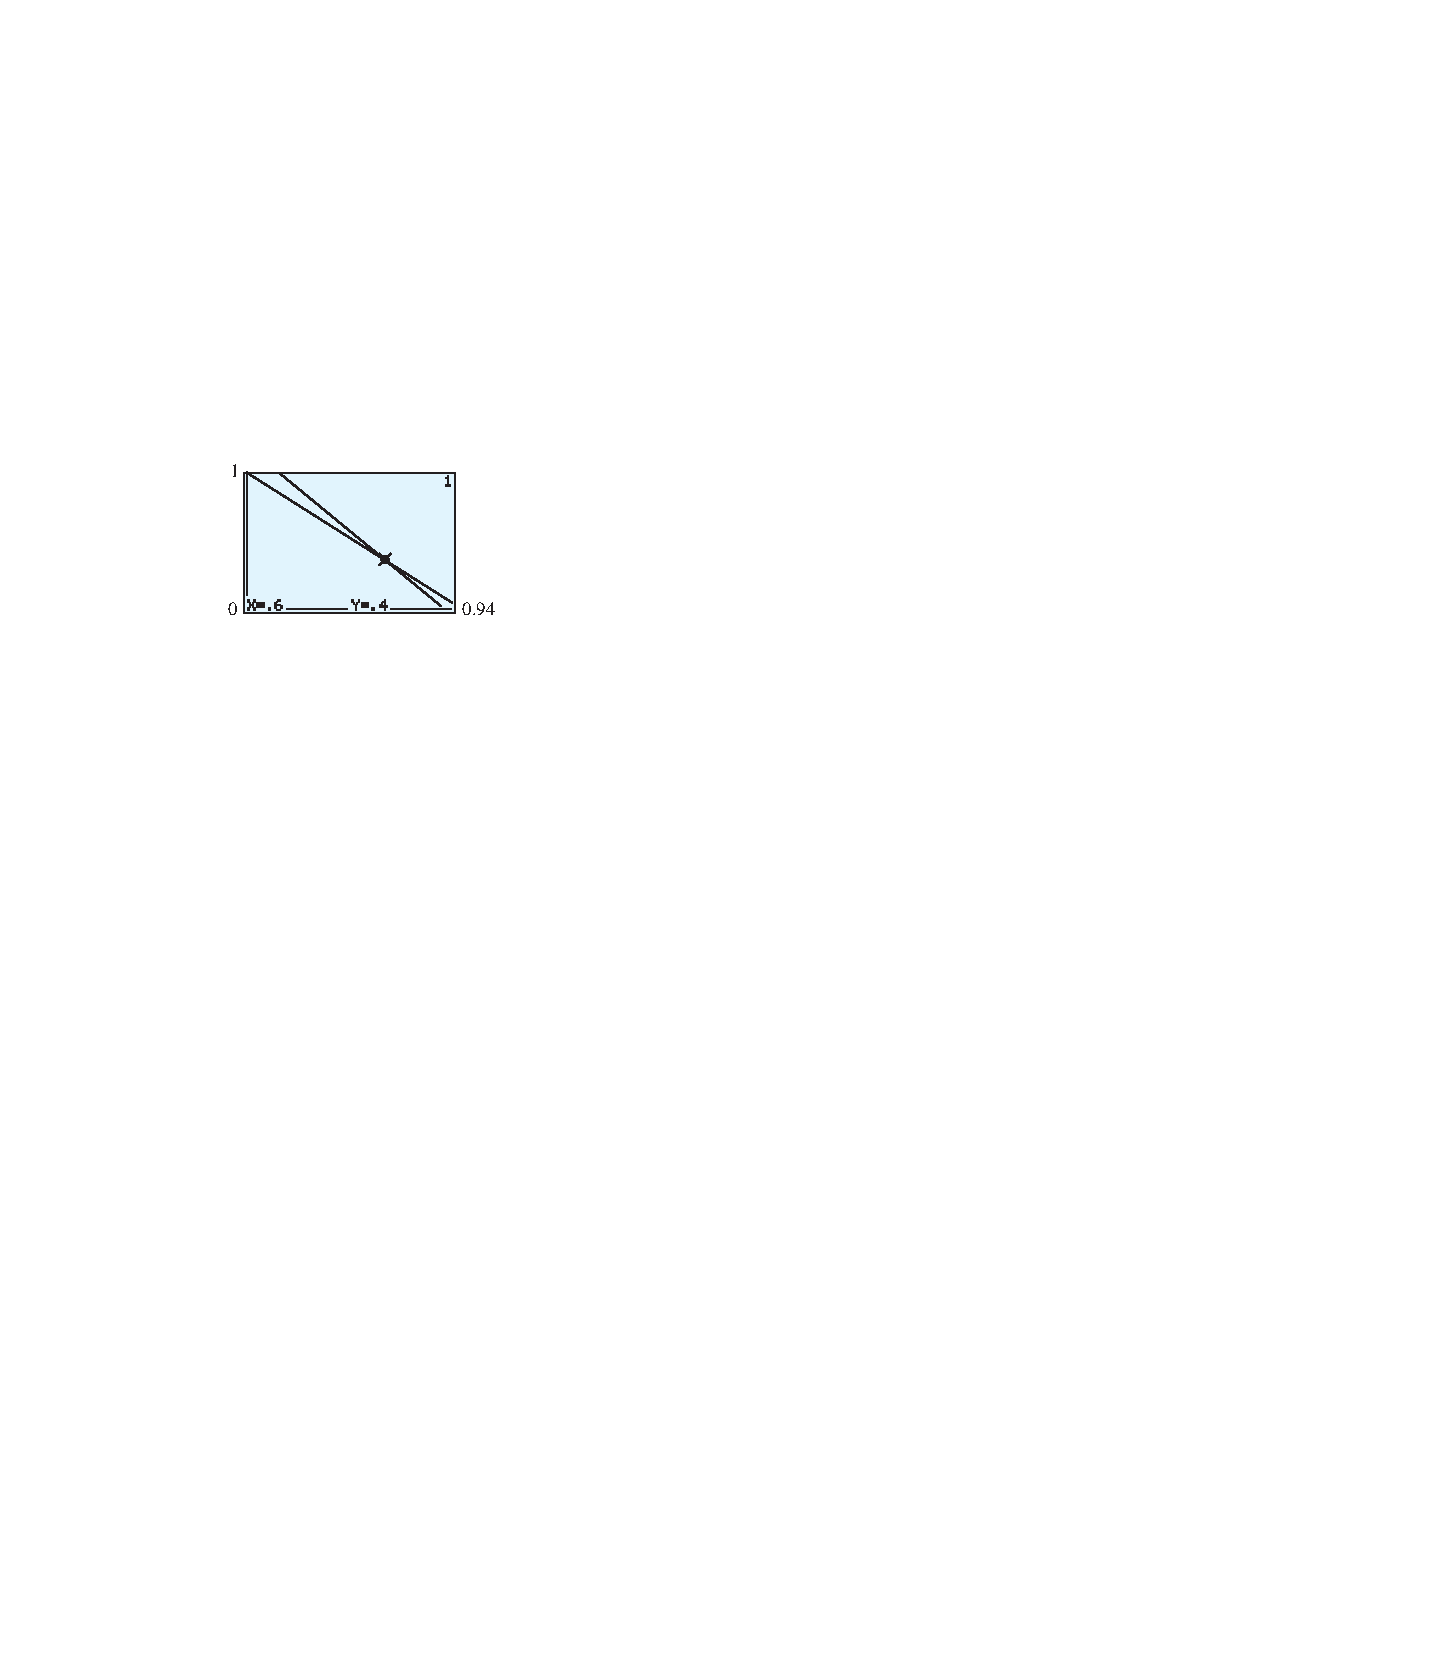
\includegraphics[width=0.50\textwidth,]{images/fig-GC-2x2-system3.pdf}\caption{\label{fig-GC-2x2-system3}}
\end{figure}

				The lines intersect at \((0.6, 0.4)\), which we can verify by substituting these values into the original two equations of our system.
			%
\item[Step 4:]{}
				Francine needs \(0.6\) cup of oats and \(0.4\) cup of wheat.
			%
\end{description}

	%
\end{example}
\begin{exercise}\label{exercise-7}

		Etienne plans to open a coffee house, and he has \(\$7520\) to spend on furniture. A table costs \(\$460\), and a chair costs \(\$120\). Etienne will buy four chairs for each table. How many tables can he buy?
		\leavevmode%
\begin{enumerate}[label=*\alph**]
\item\hypertarget{li-40}{}
				Let \(x\) represent the number of tables Etienne should buy, and let \(y\) represent the number of chairs. Write an equation about the cost of the furniture.
			%
\item\hypertarget{li-41}{}
				Write a second equation about the number of tables and chairs.
			%
\item\hypertarget{li-42}{}
				Graph both equations, solve the system, and answer the question in the problem. (Find the intercepts of the graphs to help you choose a window.)
			%
\end{enumerate}

	%
\end{exercise}
\par

	Being unable to read exact coordinates from a graph is not always a disadvantage. In many situations, fractional values of the unknowns are not acceptable.
%
\begin{example}[]\label{example-8}

		The mathematics department has \(\$40,000\) to set up a new computer lab. The department will need one printer for every four terminals it purchases. If a printer costs \(\$560\) and a terminal costs \(\$1520\), how many of each should the department buy?
	%
\par\medskip\noindent%
\textbf{Solution.}\quad 
		\leavevmode%
\begin{description}
\item[Step 1:]{}
				\begin{tabular}{ll}
Number of printers:%
&\(p\)\tabularnewline[0pt]
Number of terminals%
&\(t\)
\end{tabular}

			%
\item[Step 2:]{}
				Since the math department needs four times as many terminals as printers,
				\begin{equation*}t=4p\end{equation*}
				The total cost of the printers will be \(560p\) dollars, and the total cost of the terminals will be \(1520t\) dollars, so we have
				\begin{equation*}560p + 1520t = 40,000\end{equation*}
			%
\item[Step 3:]{}
				Solve the second equation for \(t\) to get
				\begin{equation*}t=(40,000 - 560p)/1520\end{equation*}
				Now we graph the equations
				\begin{align*}

						Y_1 \amp =4X
					\\

						Y_2 \amp =(40000 − 560X)/1520
					
\end{align*}
				on the same set of axes. The second graph is not visible in the standard graphing window, but with a little experimentation we can find an appropriate window setting. The WINDOW values used for Figure 8.8 are
				\begin{align*}

						\text{Xmin} \amp = 0 \amp\amp \text{Xmax} = 9.4
					\\

						\text{Ymin} \amp = 0 \amp\amp \text{Ymax} = 30
					
\end{align*}
				The lines intersect at approximately \((6, 24)\). These values satisfy the first equation, but not the second.
				\begin{align*}

						560(\alert{6})+1520(\blert{24})\amp\stackrel{?}{=}40,000 
					\\

						39,840 \amp\ne 40,000
					
\end{align*}
			%
\item[Step 4:]{}
				The exact solution to the system is \(\left(\frac{500}{83},\frac{2000}{83}\right)\). But this solution is not of practical use, since the math department cannot purchase fractions of printers or terminals. The department can purchase \(6\) printers and \(24\) terminals (with some money left over).
			%
\end{description}

	%
\end{example}
\begin{exercise}\label{exercise-8}

		The manager for Books for Cooks plans to spend \(\$300\) stocking a new diet cookbook. The paperback version costs her \(\$5\), and the hardback costs \(\$10\). She finds that she will sell three times as many paperbacks as hardbacks. How many of each should she buy?
		\leavevmode%
\begin{enumerate}[label=*\alph**]
\item\hypertarget{li-47}{}
				Let \(x\) represent the number of hardbacks and \(y\) the number of paperbacks she should buy. Write an equation about the cost of the books.
			%
\item\hypertarget{li-48}{}
				Write a second equation about the number of each type of book.
			%
\item\hypertarget{li-49}{}
				Graph both equations and solve the system. (Find the intercepts of the graphs to help you choose a window.) Answer the question in the problem.
			%
\end{enumerate}

	%
\end{exercise}
\typeout{************************************************}
\typeout{Subsection 1.1.4 An Application from Economics}
\typeout{************************************************}
\subsection[An Application from Economics]{An Application from Economics}\label{subsection-4}

	The owner of a retail business must try to balance the demand for his product from consumers with the supply he can obtain from manufacturers. Supply and demand both vary with the price of the product: Consumers usually buy fewer items if the price increases, but manufacturers will be willing to supply more units of the product if its price increases.
%
\par

	The \terminology{demand function} gives the number of units of the product that consumers will buy in terms of the price per unit. The \terminology{supply function} gives the number of units that the producer will supply in terms of the price per unit. The price at which the supply and demand are equal is called the \terminology{equilibrium price}. This is the price at which the consumer and the producer agree to do business.
%
\begin{example}[]\label{example-9}

		A woolens mill can produce \(400x\) yards of fine suit fabric if it can charge \(x\) dollars per yard. The mill's clients in the garment industry will buy \(6000 − 100x\) yards of wool fabric at a price of \(x\) dollars per yard. Find the equilibrium price and the amount of fabric that will change hands at that price.
	%
\par\medskip\noindent%
\textbf{Solution.}\quad 
		\leavevmode%
\begin{description}
\item[Step 1:]{}
				\begin{tabular}{ll}

							Price per yard:
						%
&\(x\)\tabularnewline[0pt]
Number of yards:%
&\(y\)
\end{tabular}

			%
\item[Step 2:]{}
				The supply equation tells us how many yards of fabric the mill will produce for a price of x dollars per yard.
				\begin{equation*}y=400x\end{equation*}
				The demand equation tells us how many yards of fabric the garment industry will buy at a price of \(x\) dollars per yard.
				\begin{equation*}y = 6000 − 100x\end{equation*}
			%
\item[Step 3:]{}
				Graph the two equations on the same set of axes, as shown in Figure 8.9. Set the window values to
				\begin{align*}

						\text{Xmin} \amp = 0 \amp\amp \text{Xmax} = 94
					\\

						\text{Ymin} \amp = 0 \amp\amp \text{Ymax} = 6200
					
\end{align*}
				and use the \lstinline?TRACE? or the \emph{intersect} command to locate the solution. the graphs intersect at the point \((12, 4800)\).
			%
\item[Step 4:]{}
				The equilibrium price is \(\$12\) per yard, and the mill will sell \(4800\) yards of fabric at that price.
			%
\end{description}

	%
\end{example}
\begin{exercise}\label{exercise-9}

		Sanaz can afford to produce \(35x\) pairs of hand-painted sunglasses if she can sell them at \(x\) dollars per pair, and the market will buy \(1700 - 15x\) at \(x\) dollars a pair.
		\leavevmode%
\begin{enumerate}[label=*\alph**]
\item\hypertarget{li-54}{}
				Write the supply and demand equations for the sunglasses.
			%
\item\hypertarget{li-55}{}
				Find the equilibrium price and the number of sunglasses Sanaz will produce and sell at that price.
			%
\end{enumerate}

	%
\end{exercise}
\typeout{************************************************}
\typeout{Section 1.2 Systems of Linear Equations in Three Variables}
\typeout{************************************************}
\section[Systems of Linear Equations in Three Variables]{Systems of Linear Equations in Three Variables}\label{Systems-of-Linear-Equations-in-Three-Variables}

	Some problems involve three (or more) unknown quantities, and efficient techniques for solving linear systems in many variables are available. In this section, we solve systems of three linear equations in three variables.
%
\typeout{************************************************}
\typeout{Subsection 1.2.1 \(3\times 3\) Linear Systems}
\typeout{************************************************}
\subsection[\(3\times 3\) Linear Systems]{\(3\times 3\) Linear Systems}\label{subsection-5}

	A solution to an equation in three variables, such as
	\begin{equation*}x + 2y − 3z = −4\end{equation*}
	is an ordered triple of numbers that satisfies the equation. For example, \((0, -2, 0)\) and \((-1, 0, 1)\) are solutions to the equation above, but \((1, 1, 1)\) is not. You can verify this by substituting the coordinates into the equation to see if a true statement results.
	\begin{alignat*}{5}

			\amp\text{For }(0,−2, 0):{}\amp 0   {}+{}\amp 2(−2) \amp{}−{}\amp 3(0) \amp = −4{}\amp\hphantom{blank} \text{True}\amp
		\\

			\amp\text{For }(−1, 0, 1):{}\amp {−}1 {}+{}\amp 2(0)  \amp{}−{}\amp 3(1) \amp = −4{}\amp\hphantom{blank} \text{True}\amp
		\\

			\amp\text{For }(1, 1, 1):{}\amp 1   {}+{}\amp 2(1)  \amp{}−{}\amp 3(1) \amp = −4{}\amp\hphantom{blank} \text{Not true}\amp 
		
\end{alignat*}
	As with the two-variable case, a single linear equation in three variables has infinitely many solutions.
%
\par

	An ordered triple \((x, y, z)\) can be represented geometrically as a point in space using a three-dimensional Cartesian coordinate system (see \hyperref[fig-3D-point]{Figure~\ref{fig-3D-point}}). In this coordinate system, the graph of a linear equation in three variables is a plane, and the fact that there are infinitely many solutions to the equation tells us that that there are infinitely many points in the corresponding plane.
%
\leavevmode%
\begin{figure}
\centering
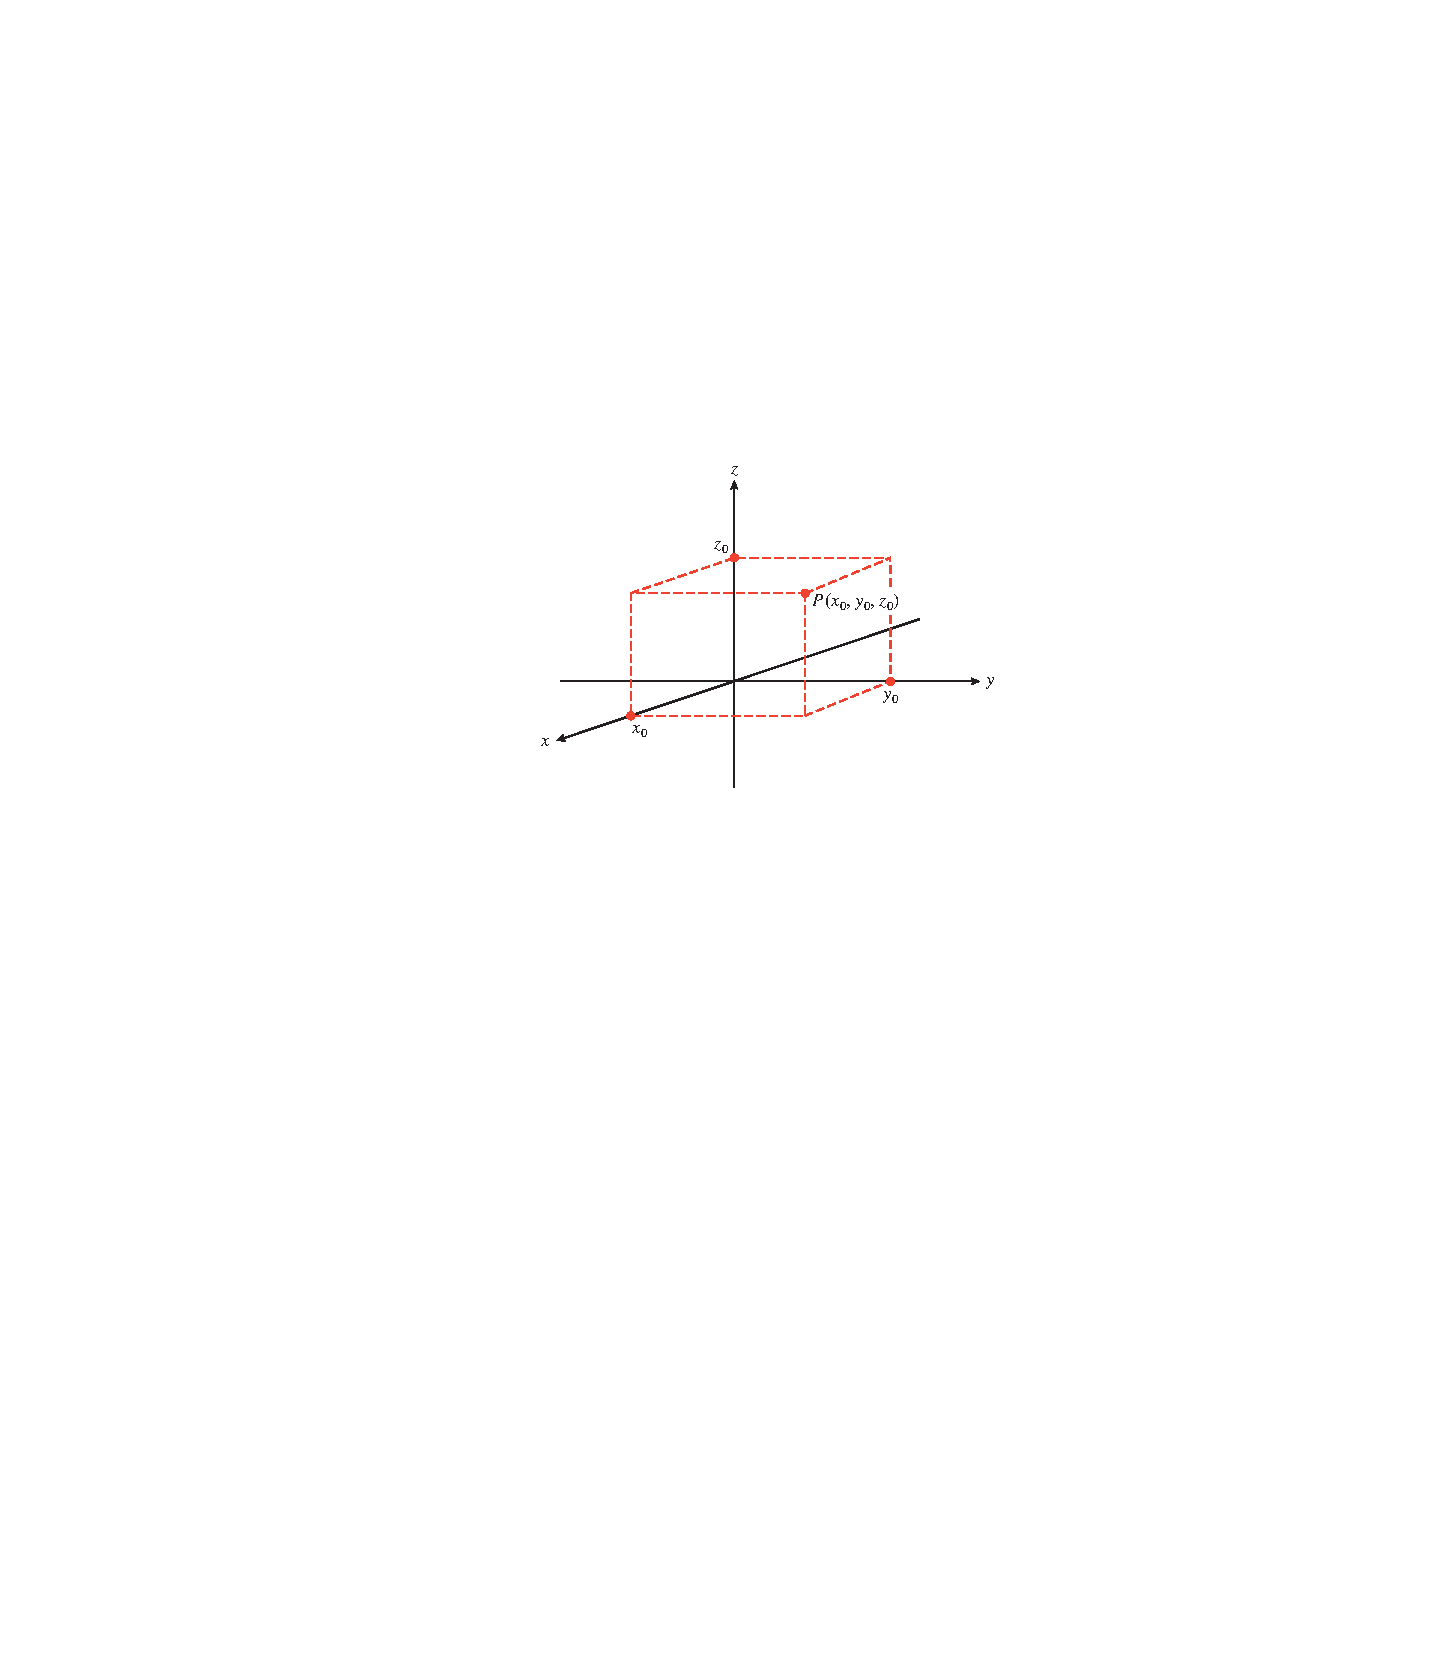
\includegraphics[,]{images/fig-3D-point.pdf}\caption{\label{fig-3D-point}}
\end{figure}
\par

	A solution to a \emph{system} of three linear equations in three variables is an ordered triple that satisfies each equation in the system. That triple represents a point that must lie on all three graphs. \hyperref[fig-8-cases-for-3-planes]{Figure~\ref{fig-8-cases-for-3-planes}} shows the different ways in which three planes may intersect in space.
%
\leavevmode%
\begin{figure}
\centering
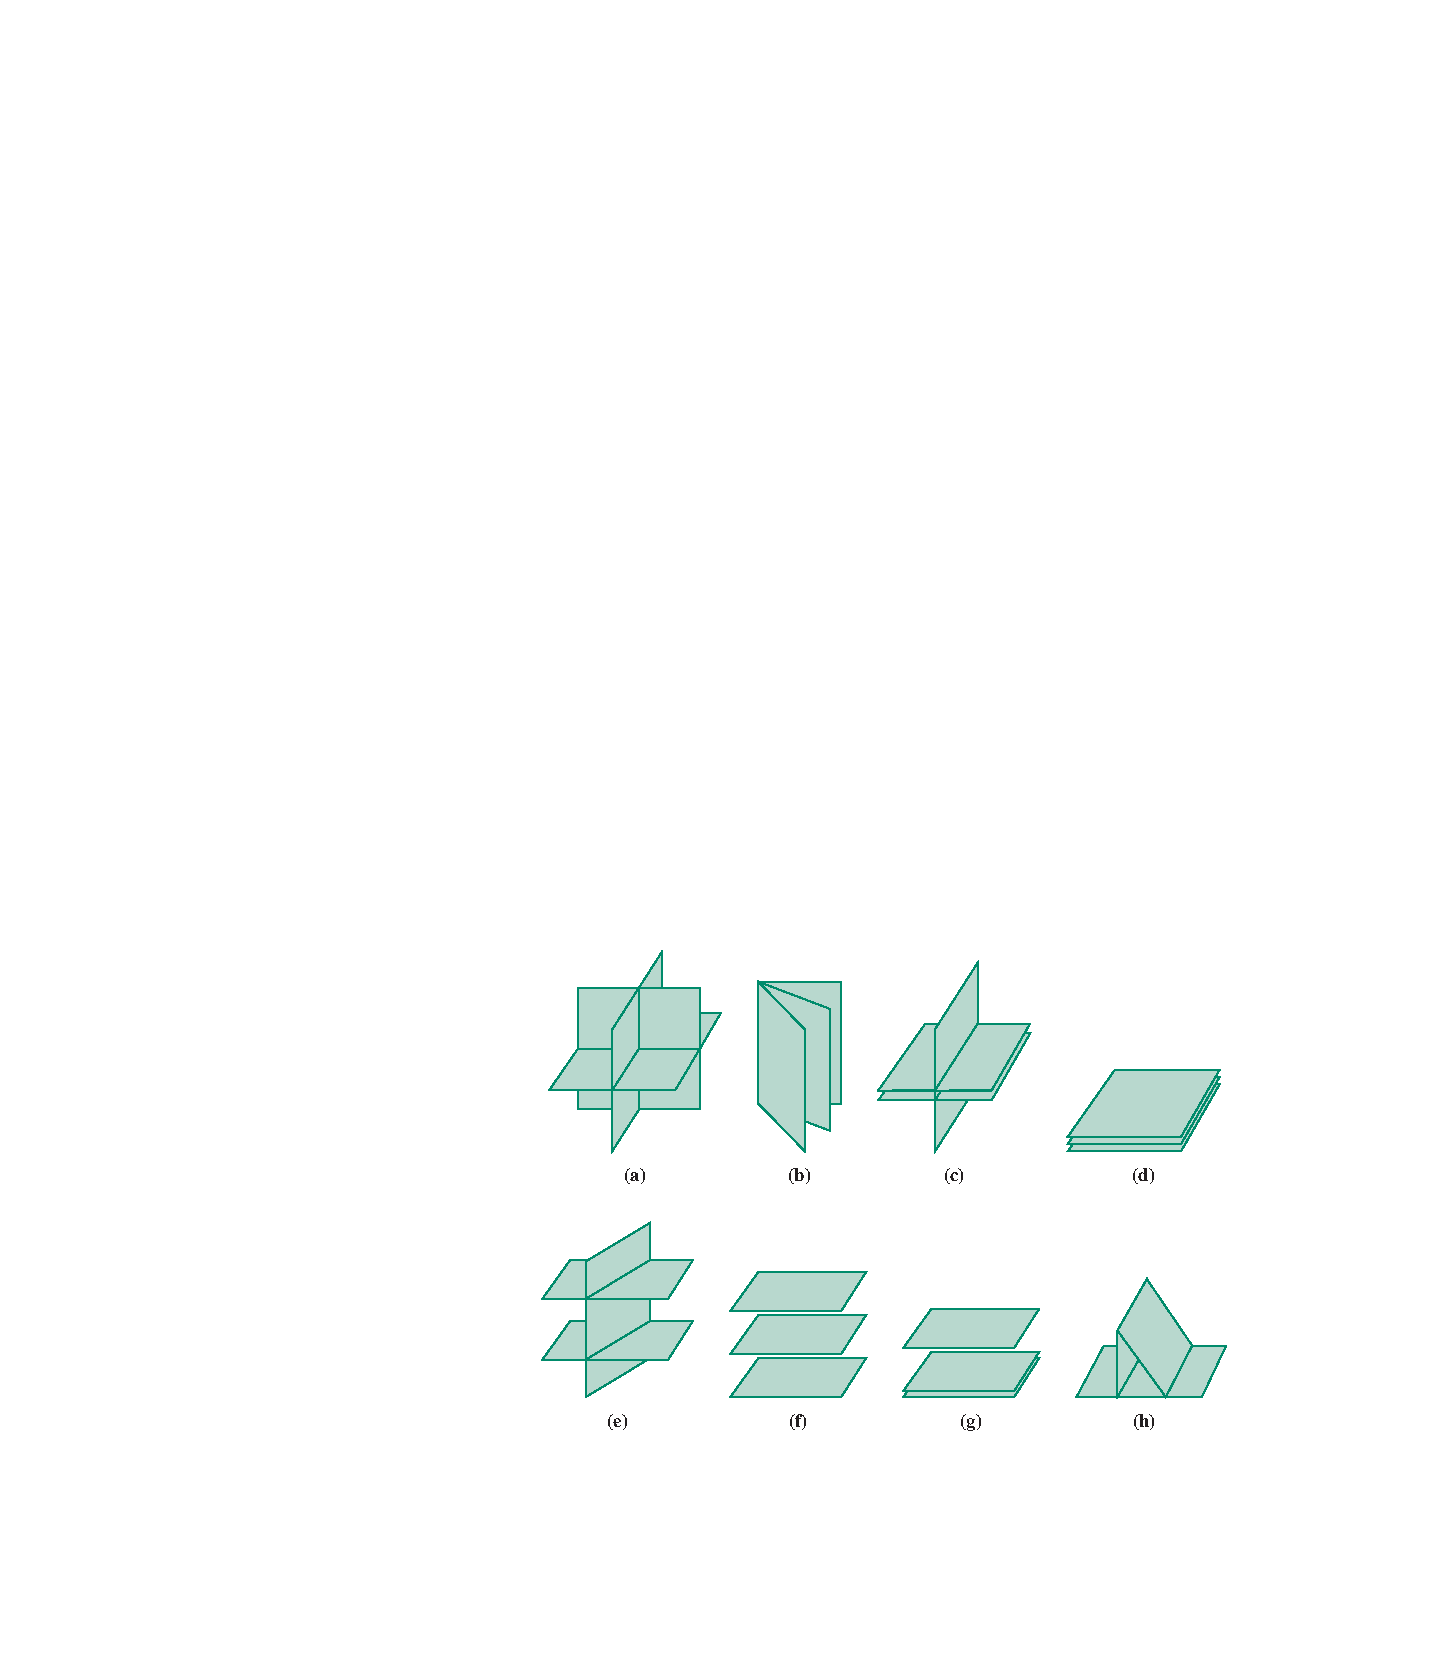
\includegraphics[,]{images/fig-8-cases-for-3-planes.pdf}\caption{\label{fig-8-cases-for-3-planes}}
\end{figure}
\par

	In \hyperref[fig-8-cases-for-3-planes]{Figure~\ref{fig-8-cases-for-3-planes}}a, the three planes intersect in a single point, so the corresponding system of three equations has a unique solution. In \hyperref[fig-8-cases-for-3-planes]{Figures~\ref{fig-8-cases-for-3-planes}}b, c, and d, the intersection is either a line or an entire plane, so the corresponding system has infinitely many solutions. Such a system is called \terminology{dependent}. In \hyperref[fig-8-cases-for-3-planes]{Figures~\ref{fig-8-cases-for-3-planes}}e, f, g, and h, the three planes have no common intersection, so the corresponding system has no solution. In this case, the system is said to be \terminology{inconsistent}.
%
\par

	It is impractical to solve \(3\times 3\) systems by graphing. Even when technology for producing three-dimensional graphs is available, we cannot read coordinates on such graphs with any confidence. Thus, we will restrict our attention to algebraic methods of solving such systems.
%
\typeout{************************************************}
\typeout{Subsection 1.2.2 Back-Substitution}
\typeout{************************************************}
\subsection[Back-Substitution]{Back-Substitution}\label{subsection-6}

	When we review our algebraic methods for \(2\times 2\) systems—substitution and linear combinations—we find features common to both. In both methods, we obtain an equation in one variable. Once we have solved for that variable, we substitute the value into an earlier equation to find the other variable.
%
\par

	One strategy for solving a \(3\times 3\) system extends this idea to include a third variable and a third equation. The following special case illustrates the substitution part of the procedure.
%
\begin{example}[]\label{example-back-substitution}

		Solve the system
		\begin{alignat*}{3}
 x +{}  2y \amp {}+{} \amp 3z \amp {}={} \amp 2\\
          -2y  \amp {}-{} \amp  4z \amp {}={} \amp -2\\
        \amp {}{} \amp 3z \amp {}={} \amp -3
\end{alignat*}
	%
\par\medskip\noindent%
\textbf{Solution.}\quad 
		The third equation involves only the variable \(z\), so we solve that equation to find \(z = −1\). Then we substitute \(-1\) for \(z\) in the second equation and solve for \(y\).
		\begin{align*}

				−2y − 4(\alert{−1}) \amp = −2
			\\

				−2y + 4 \amp= −2
			\\

				−2y \amp = −6
			\\

				y\amp=3
			
\end{align*}
		Finally, we substitute \(-1\) for \(z\) and \(3\) for \(y\) into the first equation to find \(x\).
		\begin{align*}

				x + 2(\blert{3}) + 3(\alert{−1}) \amp= 2
			\\

				x + 6 − 3 \amp = 2
			\\

				x\amp=-1
			
\end{align*}
		The solution is the ordered triple \((-1, 3, -1)\). You should verify that this triple satisfies all three equations of the system.
	%
\end{example}
\par

	The technique used in \hyperref[example-back-substitution]{Example~\ref{example-back-substitution}} is called \terminology{back-substitution}. It works in the special case where one of the equations involves exactly one variable, and a second equation involves that same variable and just one other variable. A \(3\times 3\) linear system with these properties is said to be in \terminology{triangular form}. If we can transform a system into triangular form, we can use back-substitution to complete the solution.
%
\begin{exercise}\label{exercise-10}

		Use back-substitution to solve the system
		\begin{alignat*}{3}
 2x +{}  2y \amp {}+{} \amp z \amp {}={} \amp 10\\
          y  \amp {}-{} \amp  4z \amp {}={} \amp 9\\
        \amp {}{} \amp 3z \amp {}={} \amp -6
\end{alignat*}
	%
\end{exercise}
\typeout{************************************************}
\typeout{Subsection 1.2.3 Gaussian Reduction}
\typeout{************************************************}
\subsection[Gaussian Reduction]{Gaussian Reduction}\label{subsection-7}

	We can use linear combinations to reduce a \(3\times 3\) system to triangular form and then use back-substitution to find the solutions. Our strategy will be to eliminate one of the variables from each of the three equations by considering them in pairs. This results in a \(2\times 2\) system that we can solve using elimination. As an example, consider the system
	\begin{alignat*}{4}
 x \amp {}+{} \amp 2y \amp {}-{} \amp 3z \amp {}={} \amp -4\amp\hphantom{blankblank} (1)\\
2x \amp {}-{} \amp  y \amp {}+{} \amp  z \amp {}={} \amp  3\amp\hphantom{blankblank} (2)\\
3x \amp {}+{} \amp 2y \amp {}+{} \amp  z \amp {}={} \amp 10\amp\hphantom{blankblank} (3)
\end{alignat*}
	\leavevmode%
\begin{description}
\item[Step 1: ]{}
			This system is already in standard form. We can choose any one of the three variables to eliminate first. For this example, we will eliminate \(x\).
		%
\item[Step 2:]{}
			Choose two of the equations, say (1) and (2), and use a linear combination: We multiply Equation (1) by \(-2\) and add the result to Equation (2) to produce Equation (4).
			\leavevmode%
\begin{table}
\centering
\begin{tabular}{rrrrrrrrr}
\(-2x\)&\(-\)&\(4y\)&\(+\)&\(6z\)&\(=\)&\(8\)&\(\hphantom{blank}\)&\(-2\times (1)\)\tabularnewline[0pt]
\(2x\)&\(-\)&\(y\)&\(+\)&\(z\)&\(=\)&\(3\)&\(\)&\((2)\)\tabularnewline\crulethin{1-7}
\(\)&\(\)&\(-5y\)&\(+\)&\(7z\)&\(=\)&\(11\)&\(\)&\((4)\)
\end{tabular}
\end{table}

		%
\item[Step 3:]{}
			Now we have an equation involving only two variables. But we need two equations in two unknowns to find the solution. So we choose a different pair of equations, say (1) and (3), and eliminate \(x\) again. We multiply Equation (1) by \(-3\) and add the result to Equation (3) to obtain Equation (5).
			\leavevmode%
\begin{table}
\centering
\begin{tabular}{rrrrrrrrr}
\(-3x\)&\(-\)&\(6y\)&\(+\)&\(9z\)&\(=\)&\(12\)&\(\hphantom{blank}\)&\(-3\times (1)\)\tabularnewline[0pt]
\(3x\)&\(+\)&\(2y\)&\(+\)&\(z\)&\(=\)&\(10\)&\(\)&\((3)\)\tabularnewline\crulethin{1-7}
\(\)&\(\)&\(-4y\)&\(+\)&\(10z\)&\(=\)&\(22\)&\(\)&\((5)\)
\end{tabular}
\end{table}

		%
\item[Step 4: ]{}
			We now form a \(2\times 2\) system with our new Equations (4) and (5).
			\begin{alignat*}{2}

					−5y\amp + \amp 7z \amp = 11 \hphantom{blankblank} (4)
				\\

					−4y\amp + \amp 10z \amp = 22 \hphantom{blankblank} (5)
				
\end{alignat*}
			We eliminate either \(y\) or \(z\) to obtain an equation in a single variable. If we choose to eliminate \(y\), we add \(4\) times Equation (4) to \(-5\) times Equation (5) to obtain Equation (6).
			\leavevmode%
\begin{table}
\centering
\begin{tabular}{rrrrrrr}
\(-20y\)&\(+\)&\(28z\)&\(=\)&\(44\)&\(\hphantom{blank}\)&\(4\times (4)\)\tabularnewline[0pt]
\(20y\)&\(-\)&\(50z\)&\(=\)&\(-110\)&\(\)&\(-5\times (5)\)\tabularnewline\crulethin{1-5}
\(\)&\(\)&\(-22z\)&\(=\)&\(-66\)&\(\)&\((6)\)
\end{tabular}
\end{table}

		%
\item[Step 5:]{}
			Now we can start solving for the variables. To keep things organized, we form a triangular system: Choose one of the original equations (in three variables), one of the equations from our \(2\times 2\) system, and our final equation in one variable. We choose Equations (1), (4), and (6).
		\begin{alignat*}{4}
 x \amp {}+{} \amp 2y \amp {}-{} \amp 3z \amp {}={} \amp -4\amp\hphantom{blankblank} (1)\\
\amp \amp−4y \amp+\amp 10z \amp = \amp 22 \amp\hphantom{blankblank} (5)	\\
\amp \amp     \amp\amp -22z \amp {}={} \amp -66\amp\hphantom{blankblank} (6)	
\end{alignat*}
		%
\par

			This new system is in triangular form, and it has the same solutions as the original system. We complete the solution by back-substitution. Solve Equation (6) to find \(z=3\). Substituting \(\alert{3}\) for \(z\) in Equation (4), we find
		\begin{align*}

		 		−5y + 7(\alert{3}) \amp = 11
		 	\\

		 		−5y + 21 \amp = 11
		 	\\

		 		−5y \amp = −10
		 	\\

		 		y \amp = 2
		 	
\end{align*}%
\par

		Finally, we substitute \(\alert{3}\) for \(z\) and \(\blert{2}\) for \(y\) into Equation (1) to find
		\begin{align*}

				x + 2(\blert{2}) − 3(\alert{3}) \amp = −4
			\\

				x + 4 − 9 \amp = −4
			\\

				x\amp =1
			
\end{align*}
		The solution to the system is the ordered triple \((1, 2, 3)\). You can verify that this triple satisfies all three of the original equations.
		%
\end{description}

%
\par

	The method described above for putting a linear system into triangular form is called \terminology{Gaussian reduction}, after the German mathematician Carl Gauss. We summarize our method for solving a \(3\times 3\) linear system as follows.
%
\begin{assemblage}{Steps for Solving a \(3\times 3\) Linear System}\label{assemblage-3}\par\medskip

	\leavevmode%
\begin{enumerate}[label=*\arabic**]
\item\hypertarget{li-61}{}
			Clear each equation of fractions and put it in standard form.
		%
\item\hypertarget{li-62}{}
			Choose two of the equations and eliminate one of the variables by forming a linear combination.
		%
\item\hypertarget{li-63}{}
			Choose a different pair of equations and eliminate the \emph{same} variable.
		%
\item\hypertarget{li-64}{}
			Form a \(2\times 2\) system with the equations found in steps (2) and (3). Eliminate one of the variables from this \(2\times 2\) system by using a linear combination.
		%
\item\hypertarget{li-65}{}
			Form a triangular system by choosing among the previous equations. Use back-substitution to solve the triangular system.
		%
\end{enumerate}

%
\end{assemblage}
\begin{example}[]\label{example-11}

		Solve the system
		\begin{alignat*}{4}
x\amp{}+{}\amp 2y \amp {}-{} \amp z \amp {}={} \amp -3\amp\hphantom{blankblank} (1)\\
\frac{1}{3}x \amp {}-{} \amp  y \amp {}+{} \amp\frac{1}{3}  z \amp {}={} \amp 2\amp\hphantom{blankblank} (2)\\
x \amp {}+{} \amp\frac{1}{2} y \amp {}+{} \amp  z \amp {}={} \amp\frac{5}{2} \amp\hphantom{blankblank} (3)
\end{alignat*}
	%
\par\medskip\noindent%
\textbf{Solution.}\quad 
		Follow the steps outlined above.
		\leavevmode%
\begin{description}
\item[Step 1:]{}
				Multiply each side of Equation (2) by \(3\), and multiply each side of Equation (3) by \(3\), to obtain the equivalent system		
				\begin{alignat*}{4}
x\amp{}+{}\amp 2y \amp {}-{} \amp z \amp {}={} \amp -3\amp\hphantom{blankblank} (1)\\
x \amp {}-{} \amp 3 y \amp {}+{} \amp z \amp {}={} \amp 6\amp\hphantom{blankblank} (2\text{a})\\
2x \amp {}+{} \amp y \amp {}+{} \amp  2z \amp {}={} \amp5 \amp\hphantom{blankblank} (3\text{a})
\end{alignat*}
			%
\item[Step 2:]{}
				Eliminate \(z\) from Equations (1) and (2a) by adding.
			\leavevmode%
\begin{table}
\centering
\begin{tabular}{rrrrrrrrr}
\(x\)&\(+\)&\(2y\)&\(-\)&\(z\)&\(=\)&\(-3\)&\(\hphantom{blank}\)&\((1)\)\tabularnewline[0pt]
\(x\)&\(-\)&\(3y\)&\(+\)&\(z\)&\(=\)&\(6\)&\(\)&\((2\text{a})\)\tabularnewline\crulethin{1-7}
\(2x\)&\(-\)&\(y\)&\(\)&\(\)&\(=\)&\(3\)&\(\)&\((4)\)
\end{tabular}
\end{table}

			%
\item
				Eliminate \(z\) from Equations (1) and (3a): Multiply Equation (1) by \(2\) and add the result to Equation (3a).
			\leavevmode%
\begin{table}
\centering
\begin{tabular}{rrrrrrrrr}
\(2x\)&\(+\)&\(4y\)&\(-\)&\(2z\)&\(=\)&\(-6\)&\(\hphantom{blank}\)&\((1\text{a})\)\tabularnewline[0pt]
\(2x\)&\(+\)&\(y\)&\(+\)&\(2z\)&\(=\)&\(5\)&\(\)&\((3\text{a})\)\tabularnewline\crulethin{1-7}
\(4x\)&\(+\)&\(5y\)&\(\)&\(\)&\(=\)&\(-1\)&\(\)&\((5)\)
\end{tabular}
\end{table}

			%
\item[Step 4:]{}
				Form the \(2\times 2\) system consisting of Equations (4) and (5).
				\begin{alignat*}{3}

						2x\amp {}−{}\amp y\amp =\amp 3\amp\hphantom{blankblank} (4)
					\\

						4x\amp {}+{}\amp 5y\amp =\amp −1\amp\hphantom{blankblank}  (5)
					
\end{alignat*}
			%
\item[Step 5:]{}
				Form a triangular system using Equations (1), (4), and (6).
				\begin{alignat*}{4}
 x \amp {}+{} \amp 2y \amp {}-{} \amp z \amp {}={} \amp -3\amp\hphantom{blankblank} (1)\\
2x \amp{}-{}\amp y \amp \amp  \amp = \amp 3 \amp\hphantom{blankblank} (4)	\\
\amp \amp 7y  \amp\amp  \amp {}={} \amp -7\amp\hphantom{blankblank} (6)	
\end{alignat*}
				 Use back-substitution to find the solution. You can verify that the ordered triple \((1, -1, 2)\) satisfies all three of the original equations of the system.
			%
\end{description}

	%
\end{example}
\begin{exercise}\label{exercise-11}

		Use Gaussian reduction to solve the system
		\begin{alignat*}{4}
x\amp{}-{}\amp 2y \amp {}+{} \amp z \amp {}={} \amp -1\amp\hphantom{blankblank} (1)\\
\frac{2}{3}x \amp {}+{} \amp \frac{1}{3}y \amp {}-{} \amp z \amp {}={} \amp 1\amp\hphantom{blankblank} (2)\\
3x \amp {}+{} \amp 3y \amp {}-{} \amp 2z \amp {}={} \amp 10 \amp\hphantom{blankblank} (3)
\end{alignat*}
		Follow the steps suggested below:
		\leavevmode%
\begin{enumerate}[label=*\arabic**]
\item\hypertarget{li-71}{}
				Clear the fractions from Equation (2).
			%
\item\hypertarget{li-72}{}
				Eliminate \(z\) from Equations (1) and (2).
			%
\item\hypertarget{li-73}{}
				Eliminate \(z\) from Equations (1) and (3).
			%
\item\hypertarget{li-74}{}
				Eliminate \(x\) from your new \(2\times 2\) system.
			%
\item\hypertarget{li-75}{}
				Form a triangular system and solve by back-substitution.
			%
\end{enumerate}

	%
\end{exercise}
\typeout{************************************************}
\typeout{Subsection 1.2.4 Inconsistent and Dependent Systems}
\typeout{************************************************}
\subsection[Inconsistent and Dependent Systems]{Inconsistent and Dependent Systems}\label{subsection-8}

	The results in \hyperref[Systems-of-Linear-Equations-in-Two-Variables]{Section~\ref{Systems-of-Linear-Equations-in-Two-Variables}} for identifying dependent and inconsistent systems can be extended to \(3\times 3\) linear systems. If at any step in forming linear combinations we obtain an equation of the form
	\begin{equation*}
		0x + 0y + 0z = k, \hphantom{blank}(k\ne 0)
	\end{equation*}
	then the system is inconsistent and has no solution. If we obtain an equation of the form
	\begin{equation*}
		0x + 0y + 0z = 0
	\end{equation*}
	then the system is dependent and has infinitely many solutions.
%
\begin{example}[]\label{example-12}

		Solve the system
		\begin{alignat*}{5}

				3x\amp {}+{}\amp y\amp {}−{}\amp 2z\amp =\amp 1\amp\hphantom{blank} \amp(1)
			\\

				6x\amp {}+{}\amp 2y\amp {}−{}\amp 4z\amp =\amp 5\amp\hphantom{blank} \amp(2)
			\\

				−2x\amp {}−{}\amp y\amp {}+{}\amp 3z\amp =\amp −1\amp\hphantom{blank} \amp(3)
			
\end{alignat*}
	%
\par\medskip\noindent%
\textbf{Solution.}\quad 
		To eliminate \(y\) from Equations (1) and (2), multiply Equation (1) by \(-2\) and add the result to Equation (2).
		\leavevmode%
\begin{table}
\centering
\begin{tabular}{rrrrrrr}
\(-6x\)&\(-\)&\(2y\)&\(+\)&\(4z\)&\(=\)&\(-2\)\tabularnewline[0pt]
\(6x\)&\(+\)&\(2y\)&\(-\)&\(4z\)&\(=\)&\(5\)\tabularnewline\crulethin{1-5}\crulethin{7-7}
\(0x\)&\(+\)&\(0y\)&\(+\)&\(0z\)&\(=\)&\(3\)
\end{tabular}
\end{table}



		Since the resulting equation has no solution, the system is \emph{inconsistent}.
	%
\end{example}
\begin{exercise}\label{exercise-12}

		Decide whether the system is inconsistent, dependent, or consistent and independent.
		\begin{alignat*}{4}

				x\amp {}+{}\amp 3y\amp {}−{}\amp z\amp =\amp 4 
			\\

				-2x\amp {}-{}\amp 6y\amp {}+{}\amp 2z\amp =\amp 1 
			\\

				x\amp {}+{}\amp 2y\amp {}-{}\amp z\amp =\amp 3 
			
\end{alignat*}
	%
\end{exercise}
\begin{example}[]\label{example-13}

		Solve the system
		\begin{alignat*}{5}

				-x\amp {}+{}\amp 3y\amp {}−{}\amp z\amp =\amp -2\amp\hphantom{blank} \amp(1)
			\\

				2x\amp {}+{}\amp y\amp {}-{}\amp 4z\amp =\amp 6\amp\hphantom{blank} \amp(2)
			\\

				2x\amp {}-{}\amp 6y\amp {}+{}\amp 2z\amp =\amp 4\amp\hphantom{blank} \amp(3)
			
\end{alignat*}
	%
\par\medskip\noindent%
\textbf{Solution.}\quad 
		To eliminate \(x\) from Equations (1) and (3), multiply Equation (1) by 2 and add Equation (3).
		\leavevmode%
\begin{table}
\centering
\begin{tabular}{rrrrrrr}
\(-2x\)&\(+\)&\(6y\)&\(-\)&\(2z\)&\(=\)&\(-4\)\tabularnewline[0pt]
\(2x\)&\(-\)&\(6y\)&\(+\)&\(2z\)&\(=\)&\(4\)\tabularnewline\crulethin{1-5}\crulethin{7-7}
\(0x\)&\(+\)&\(0y\)&\(+\)&\(0z\)&\(=\)&\(0\)
\end{tabular}
\end{table}

		Since the resulting equation vanishes, the system is dependent and has infinitely many solutions.
	%
\end{example}
\begin{exercise}\label{exercise-13}

		Decide whether the system is inconsistent, dependent, or consistent and independent.
		\begin{align*}

				a − c \amp = 2
			\\

				2a + b \amp = 5
			\\

				a + b + c = 3
			
\end{align*}
	%
\end{exercise}
\typeout{************************************************}
\typeout{Subsection 1.2.5 Applications}
\typeout{************************************************}
\subsection[Applications]{Applications}\label{subsection-9}

	Here are some problems that can be modeled by a system of three linear equations. When writing such systems, we must be careful to find three independent equations describing the conditions of the problem.
%
\begin{example}[]\label{example-14}

		One angle of a triangle measures 4° less than twice the second angle, and the third angle is 20° greater than the sum of the first two. Find the measure of each angle.
	%
\par\medskip\noindent%
\textbf{Solution.}\quad 
		\leavevmode%
\begin{description}
\item[Step 1: ]{}
				Represent the measure of each angle by a separate variable.
				\begin{align*}

						\amp\text{First angle: }\amp\amp x
					\\

						\amp\text{Second angle: }\amp\amp y
					\\

						\amp\text{Third angle:}\amp\amp z
					
\end{align*}
			%
\item[Step 2:]{}
				Write the conditions stated in the problem as three equations.
				\begin{gather*}
x = 2y − 4\\
z = x + y + 20\\
x + y + z = 180
\end{gather*}
				(The third equation states the fact that the sum of the angles of a triangle is 180°.)
			%
\item[Step 3:]{}
				We follow the steps for solving a \(3\times 3\) linear system.
				1. 		Write the three equations in standard form.
						\begin{alignat*}{5}

								x\amp {}-{}\amp 2y\amp {}{}\amp \amp =\amp -4\amp\hphantom{blank} \amp(1)
							\\

								x\amp {}+{}\amp y\amp {}-{}\amp z\amp =\amp -20\amp\hphantom{blank} \amp(2)
							\\

								x\amp {}+{}\amp y\amp {}+{}\amp z\amp =\amp 180\amp\hphantom{blank} \amp(3)
							
\end{alignat*}		
				%

				\par

					2-3. Since Equation (1) has no \(z\)-term, it will be most efficient to eliminate the variable \(z\) from Equations (2) and (3). Add these two equations.
		\leavevmode%
\begin{table}
\centering
\begin{tabular}{rrrrrrrrr}
\(x\)&\(+\)&\(y\)&\(-\)&\(z\)&\(=\)&\(-20\)&&\((2)\)\tabularnewline[0pt]
\(x\)&\(+\)&\(y\)&\(+\)&\(2z\)&\(=\)&\(4\)&&\((3)\)\tabularnewline\crulethin{1-5}\crulethin{7-7}
\(2x\)&\(+\)&\(2y\)&\(\)&\(\)&\(=\)&\(160\)&&\((4)\)
\end{tabular}
\end{table}

				%

				\par

					4. Form a \(2\times 2\) system from Equations (1) and (4). Add the two equations to eliminate the variable \(y\), yielding
		\leavevmode%
\begin{table}
\centering
\begin{tabular}{rrrrrrr}
\(x\)&\(-\)&\(2y\)&\(=\)&\(-4\)&&\((1)\)\tabularnewline[0pt]
\(2x\)&\(+\)&\(2y\)&\(=\)&\(160\)&&\((4)\)\tabularnewline\crulethin{1-3}\crulethin{5-5}
\(3x\)&\(\)&\(\)&\(=\)&\(156\)&&\((5)\)
\end{tabular}
\end{table}

				%

				\par

					5. Form a triangular system using Equations (3), (1), and (5). Use back-substitution to complete the solution.
					\begin{alignat*}{4}

							x\amp {}+{}\amp y\amp {}+{}\amp z\amp =\amp 180\hphantom{blankblank} \amp(2)
						\\

							x\amp {}−{}\amp 2y\amp \amp\amp =\amp −4\hphantom{blankblank} \amp(1)
						\\

							3x\amp\amp\amp\amp\amp = \amp156\hphantom{blankblank} \amp(5)
						
\end{alignat*}
					Divide both sides of Equation (5) by \(3\) to find \(x = 52\). Substitute \(52\) for \(x\) in Equation (1) and solve for \(y\) to find
					\begin{align*}

							\alert{52} − 2y \amp = −4
						\\

							y \amp= 28
						
\end{align*}
					Substitute \(52\) for \(x\) and \(28\) for \(y\) in Equation (3) to find
					\begin{align*}

							\alert{52} + \blert{28} + z \amp= 180
						\\

							z\amp=100
						
\end{align*}
				%

			%
\item[Step 4:]{}
				The angles measure 52°, 28°, and 100°.
			%
\end{description}

	%
\end{example}
\begin{exercise}\label{exercise-14}

		A manufacturer of office supplies makes three types of file cabinet: two-drawer, four-drawer, and horizontal. The manufacturing process is divided into three phases: assembly, painting, and finishing. A two-drawer cabinet requires 3 hours to assemble, 1 hour to paint, and 1 hour to finish. The four-drawer model takes 5 hours to assemble, 90 minutes to paint, and 2 hours to finish. The horizontal cabinet takes 4 hours to assemble, 1 hour to paint, and 3 hours to finish. The manufacturer employs enough workers for 500 hours of assembly time, 150 hours of painting, and 230 hours of finishing per week. How many of each type of file cabinet should he make in order to use all the hours available?
		\leavevmode%
\begin{description}
\item[Step 1:]{}
				Represent the number of each model of file cabinet by a different variable.
				\leavevmode%
\begin{table}
\centering
\begin{tabular}{ll}
Number of two-drawer cabinets:%
&\(x\)\tabularnewline[0pt]
Number of four-drawer cabinets:%
&\(y\)\tabularnewline[0pt]
Number of horizontal cabinets:%
&\(z\)
\end{tabular}
\end{table}

			%
\item[Step 2:]{}
				Organize the information into a table. (Convert all times to hours.)
				\leavevmode%
\begin{table}
\centering
\begin{tabular}{AcAcAcAcAcA}\hrulethick
\(\)&2-Drawer%
&4-Drawer%
&Horizontal%
&Total available%
\tabularnewline\hrulethin
Assembly%
&\(\)&\(\)&\(\)&\(\)\tabularnewline\hrulethin
Painting%
&\(\)&\(\)&\(\)&\(\)\tabularnewline\hrulethin
Finishing%
&\(\)&\(\)&\(\)&\(\)\tabularnewline\hrulethin
\end{tabular}
\end{table}

				Write three equations describing the time constraints in each of the three manufacturing phases. For example, the assembly phase requires \(3x\) hours for the two-drawer cabinets, \(5y\) hours for the four-drawer cabinets, and \(4z\) hours for the horizontal cabinets, and the sum of these times should be the time available, \(500\) hours.
				\leavevmode%
\begin{table}
\centering
\begin{tabular}{lll}

							Assembly time:
						&\fillin{11.3636363636364}%
&\((1)\)\tabularnewline[0pt]

							Painting time:
						&\fillin{11.3636363636364}%
&\((2)\)\tabularnewline[0pt]

							Finishing time:
						&\fillin{11.3636363636364}%
&\((3)\)
\end{tabular}
\end{table}

			%
\item[Step 3:]{}
				Solve the system. Follow the steps suggested below.
				\begin{enumerate}[label=*\arabic**]
\item\hypertarget{li-83}{}
						Clear the fractions from the second equation.
					%
\item\hypertarget{li-84}{}
						Subtract Equation (1) from \(3\) times Equation (3) to obtain a new Equation (4).
					%
\item\hypertarget{li-85}{}
						Subtract Equation (2) from twice Equation (3) to obtain a new Equation (5).
					%
\item\hypertarget{li-86}{}
						Equations (4) and (5) form a \(2\times 2\) system in \(y\) and \(z\). Subtract Equation (5) from Equation (4) to obtain a new Equation (6).
					%
\item\hypertarget{li-87}{}
						Form a triangular system with Equations (3), (4), and (6). Use back-substitution to complete the solution.
					%
\end{enumerate}

			%
\item[Step 4:]{}
				You should have found the following solution: The manufacturer should make \(60\) two-drawer cabinets, \(40\) four-drawer cabinets, and \(30\) horizontal cabinets.
			%
\end{description}

	%
\end{exercise}
%
%% A lineskip in table of contents as transition to appendices, backmatter
\addtocontents{toc}{\vspace{\normalbaselineskip}}
%
%
\appendix
%
\typeout{************************************************}
\typeout{Appendix A Algebra Skills Refresher}
\typeout{************************************************}
\chapter[Algebra Skills Refresher]{Algebra Skills Refresher}\label{appendix-1}
\typeout{************************************************}
\typeout{Section A.1 Order of Operations}
\typeout{************************************************}
\section[Order of Operations]{Order of Operations}\label{Order-of-Operations}
Numerical calculations often involve more than one operation. So that everyone agrees on how such expressions should be evaluated, we follow the order of operations.%
\typeout{************************************************}
\typeout{Section A.2 Linear Equations and Inequalities}
\typeout{************************************************}
\section[Linear Equations and Inequalities]{Linear Equations and Inequalities}\label{appendix-Linear-Equations-and-Inequalities}
An \terminology{equation} is just a mathematical statement that two expressions are equal. Equations relating two variables are particularly useful. If we know the value of one of the variables, we can find the corresponding value of the other variable by solving the equation.%
\typeout{************************************************}
\typeout{Section A.3 Algebraic Expressions and Problem Solving}
\typeout{************************************************}
\section[Algebraic Expressions and Problem Solving]{Algebraic Expressions and Problem Solving}\label{appendix-Algebraic-Expressions-and-Problem-Solving}
You are familiar with the use of letters, or \terminology{variables}, to stand for unknown numbers in equations or formulas. Variables are also used to represent numerical quantities that change over time or in different situations. For example, \(p\) might stand for the atmospheric pressure at different heights above the Earth's surface. Or \(N\) might represent the number of people infected with cholera \(t\) days after the start of an epidemic.%
\typeout{************************************************}
\typeout{Section A.4 Graphs and Equations}
\typeout{************************************************}
\section[Graphs and Equations]{Graphs and Equations}\label{appendix-Graphs-and-Equations}
Graphs are useful tools for studying mathematical relationships. A graph provides an overview of a quantity of data, and it helps us identify trends or unexpected occurrences. Interpreting the graph can help us answer questions about the data.%
\typeout{************************************************}
\typeout{Section A.5 Linear Systems in Two Variables}
\typeout{************************************************}
\section[Linear Systems in Two Variables]{Linear Systems in Two Variables}\label{appendix-Linear-Systems-in-Two-Variables}
\index{}A \(2\times 2\) \terminology{system} of equations is a set of \(2\) equations in the same \(2\) variables. A \terminology{solution} of a \(2\times 2\) system is an ordered pair that makes each equation in the system true. In this section, we review two algebraic methods for solving \(2\times 2\) linear systems: substitution and elimination.%
\typeout{************************************************}
\typeout{Section A.6 Laws of Exponents}
\typeout{************************************************}
\section[Laws of Exponents]{Laws of Exponents}\label{appendix-Laws-of-Exponents}
\index{}In this section, we review the rules for performing operations on powers.%
\typeout{************************************************}
\typeout{Section A.7 Polynomials and Factoring}
\typeout{************************************************}
\section[Polynomials and Factoring]{Polynomials and Factoring}\label{appendix-Polynomials-and-Factoring}
In \hyperref[appendix-Laws-of-Exponents]{Section~\ref{appendix-Laws-of-Exponents}}, we used the first law of exponents to multiply two or more monomials. In this section, we review techniques for multiplying and factoring polynomials of several terms.%
\typeout{************************************************}
\typeout{Section A.8 Factoring Quadratic Trinomials}
\typeout{************************************************}
\section[Factoring Quadratic Trinomials]{Factoring Quadratic Trinomials}\label{appendix-Factoring-Quadratic-Trinomials}
Consider the trinomial
            \begin{equation*}
                x^2 + 10x + 16
            \end{equation*}
        %
\typeout{************************************************}
\typeout{Section A.9 Working with Algebraic Fractions}
\typeout{************************************************}
\section[Working with Algebraic Fractions]{Working with Algebraic Fractions}\label{appendix-Working-with-Algebraic-Fractions}

            A quotient of two polynomials is called a \terminology{rational expression} or an \terminology{algebraic fraction}. Operations on algebraic fractions follow the same rules as operations on common fractions.
        %
\typeout{************************************************}
\typeout{Section A.10 Working with Radicals}
\typeout{************************************************}
\section[Working with Radicals]{Working with Radicals}\label{appendix-Working-with-Radicals}
In some situations, radical notation is more convenient to use than exponents. In these cases, we usually simplify radical expressions algebraically as much as possible before using a calculator to obtain decimal approximations.%
\typeout{************************************************}
\typeout{Section A.11 Facts from Geometry}
\typeout{************************************************}
\section[Facts from Geometry]{Facts from Geometry}\label{appendix-Facts-from-Geometry}

            In this section, we review some information you will need from geometry. You are already familiar with the formulas for the area and perimeter of common geometric figures; you can find these formulas in the reference section at the front of the book.
        %
\typeout{************************************************}
\typeout{Section A.12 The Real Number System}
\typeout{************************************************}
\section[The Real Number System]{The Real Number System}\label{appendix-The-Real-Number-System}
\typeout{************************************************}
\typeout{Subsection A.12.1 Subsets of the Real Numbers}
\typeout{************************************************}
\subsection[Subsets of the Real Numbers]{Subsets of the Real Numbers}\label{subsection-10}

            The numbers associated with points on a number line are called the \terminology{real numbers}. The set of real numbers is denoted by \(\mathbb{R}\). You are already familiar with several types, or subsets, of real numbers:
        %
\typeout{************************************************}
\typeout{Appendix B Using a Graphing Calculator}
\typeout{************************************************}
\chapter[Using a Graphing Calculator]{Using a Graphing Calculator}\label{appendix-2}
\typeout{************************************************}
\typeout{Introduction  }
\typeout{************************************************}
This appendix provides instructions for TI-84 or TI-83 calculators from Texas Instruments, but most other calculators work similarly.We describe only the basic operations and features of the graphing calculator used in your textbook.%
\typeout{************************************************}
\typeout{Section B.1 Getting Started}
\typeout{************************************************}
\section[Getting Started]{Getting Started}\label{appendix-Getting-Started}
\typeout{************************************************}
\typeout{Subsection B.1.1 On and Off}
\typeout{************************************************}
\subsection[On and Off]{On and Off}\label{subsection-11}

            Press \lstinline?ON? to turn \emph{on} the calculator (see Figure B.1a). You will see a cursor blinking in the upper left corner of the Home screen. Press \lstinline?2nd?\lstinline?ON? to turn \emph{off} the calculator.
        %
\typeout{************************************************}
\typeout{Section B.2 Entering Expressions}
\typeout{************************************************}
\section[Entering Expressions]{Entering Expressions}\label{appendix-Entering-Expressions}
\typeout{************************************************}
\typeout{Section B.3 Editing Expressions}
\typeout{************************************************}
\section[Editing Expressions]{Editing Expressions}\label{appendix-Editing-Expressions}
\typeout{************************************************}
\typeout{Section B.4 Graphing an Equation}
\typeout{************************************************}
\section[Graphing an Equation]{Graphing an Equation}\label{appendix-Graphing-an-Equation}
\typeout{************************************************}
\typeout{Section B.5 Making a Table}
\typeout{************************************************}
\section[Making a Table]{Making a Table}\label{appendix-Making-a-Table}
\typeout{************************************************}
\typeout{Section B.6 Regression}
\typeout{************************************************}
\section[Regression]{Regression}\label{appendix-Regression}
\typeout{************************************************}
\typeout{Section B.7 Function Notation and Transformation of Graphs}
\typeout{************************************************}
\section[Function Notation and Transformation of Graphs]{Function Notation and Transformation of Graphs}\label{appendix-Function-Notation-and-Transformation-of-Graphs}
\typeout{************************************************}
\typeout{Appendix C Glossary}
\typeout{************************************************}
\chapter[Glossary]{Glossary}\label{appendix-3}
\typeout{************************************************}
\typeout{Appendix D Answers to selected exercises}
\typeout{************************************************}
\chapter[Answers to selected exercises]{Answers to selected exercises}\label{appendix-4}
%
\backmatter
%
%
%% The index is here, setup is all in preamble
\printindex
%
\cleardoublepage
\pagestyle{empty}
\vspace*{\stretch{1}}
\centerline{This book was authored in MathBook XML.%
}
\vspace*{\stretch{2}}
%
%% The index is here, setup is all in preamble
\printindex
%
\end{document}